\documentclass[11pt]{report}

% Packages
\usepackage{graphicx}     % For images
\usepackage{fancyhdr}     % For headers and footers
\usepackage[top=2.5cm, left=2.5cm, right=2.5cm, bottom=2.5cm, headheight=1.25cm, footskip=1.25cm]{geometry} % Page Margins
\usepackage{iflang}       % For language conditional commands
\usepackage{polyglossia}  % For multiple languages
\usepackage{fontspec}     % For specifying fonts
\usepackage{indentfirst}
\usepackage{caption}
\usepackage{subcaption}
\usepackage{dirtytalk}
\usepackage{braket}
\usepackage{minted}
\usemintedstyle{friendly}
\setmintedinline{breaklines}
\usepackage{amsmath}
\usepackage{amsfonts}
\usepackage[numbib]{tocbibind}
\usepackage{hyperref}
\usepackage{circuitikz}
\usepackage{epigraph}

\usepackage{todonotes} % remove after "realese"


%=================================================================
% Language settings, switch the two languages to change language.
\setdefaultlanguage{english} % Default language is English
\setotherlanguage{greek}     % Secondary language is Greek

% Document-specific information
\newcommand{\thesisTitle}{Implementing a Quantum Arithmetic Logic Unit using the Qiskit SDK}
\newcommand{\thesisTitleGreek}{Υλοποιώντας μια Κβαντική Αριθμητική Λογική Μονάδα με το Qiskit SDK}
\newcommand{\thesisID}{23167}
\newcommand{\studentName}{Athanasios Tzimas}
\newcommand{\studentNameGreek}{Αθανάσιος Τζίμας}
\newcommand{\studentID}{185287}
\newcommand{\supervisorName}{Ioannis K. Marmorkos}
\newcommand{\supervisorNameGreek}{Ιωάννης Κ. Μαρμόρκος}
\newcommand{\undertakingDate}{23-04-2023}
\newcommand{\completionDate}{25-05-2024}
%=================================================================

% Font settings
\setmainfont{FreeSerif} % Main font is FreeSerif
\setsansfont{FreeSans}  % Sans Serif font is FreeSans
\setmonofont{FreeMono}  % Monospaced font is FreeMono
\newfontfamily\headerfont[Scale=0.95]{FreeSerif} % Font for headers and footers

% Paragraph settings
\setlength{\parskip}{10pt}  % Paragraph spacing
\setlength{\parindent}{0cm} % Paragraph indentation

% -----------------------------------
% Header and footer settings
% -----------------------------------
\pagestyle{fancy}
\fancyhf{} % Clear all header and footer fields
\fancyhead[R]{\headerfont\nouppercase{\leftmark}} % Chapter name on right side with headerfont font
\fancyfoot[C]{\headerfont\thepage} % Page number at center with headerfont font

% -----------------------------------
% Document content
% -----------------------------------
\begin{document}

% Front Matter
\pagenumbering{roman} % Roman numerals for front matter
\begin{titlepage}
\centering

\includegraphics[width=10cm]{images/titlepage/ihu-logo-gr.png}

\IfLanguageName{greek}{
    % This content will be shown when the language is set to Greek
    \textsc{\huge Διεθνές Πανεπιστήμιο Ελλάδος}\\
    \textsc{\large Tμήμα Μηχανικών Πληροφορικής και Ηλεκτρονικών Συστημάτων}

    \vspace{2cm}

    \textbf{\Large ΔΙΠΛΩΜΑΤΙΚΗ ΕΡΓΑΣΙΑ}\\
    \vspace{0.5cm}
    \textbf{\LARGE \thesisTitleGreek}

    \vspace{1.5cm}

    \includegraphics[width=14cm]{images/titlepage/Cover-Image-Placeholder.png}

    \vspace{50pt}

    \begin{minipage}[t]{0.45\textwidth}
    \raggedright
    \textbf{Φοιτητής:}\\
    \studentNameGreek\\
    Αριθμός Μητρώου: \studentID
    \end{minipage}
    \hspace{1cm}
    \begin{minipage}[t]{0.45\textwidth}
    \raggedleft
    \textbf{Επιβλέπων:}\\
    \supervisorNameGreek\\
    \end{minipage}

    \vfill
    {23 Μαΐου 2023}
}{
    % This content will be shown when the language is set to English
    \textsc{\huge International Hellenic University}\\
    \textsc{\large Department of Information and Electronic Engineering}

    \vspace{2cm}

    \textbf{\Large THESIS}\\
    \vspace{0.5cm}
    \textbf{\LARGE \thesisTitle}

    \vspace{1.5cm}

    \vspace{50pt}

    \begin{minipage}[t]{0.45\textwidth}
    \raggedright
    \textbf{Student:}\\
    \studentName\\
    Student ID: \studentID
    \end{minipage}
    \hspace{1cm}
    \begin{minipage}[t]{0.45\textwidth}
    \raggedleft
    \textbf{Supervisor:}\\
    \supervisorName\\
    \end{minipage}

    \vfill
    { \today}
}
\end{titlepage}

\thispagestyle{empty} % hide chapter header

\vspace{3cm}

\begin{center}
Title of Dissertation \thesisTitle\\
Code of Dissertation \thesisID\\
Student’s full name \studentName\\\
Supervisor’s full name \supervisorName\\\
Date of undertaking \undertakingDate\\
Date of completion \completionDate\\
\end{center}

We hereby affirm the authorship of this paper as well as the acknowledgement and credit of whichever assistance We received in its composition. We have, furthermore, noted the various sources from which We extracted data, ideas, visual or written material, in paraphrase or exact quotation. Moreover, we affirm the exclusive composition of this paper by myself only, for the purpose of it being a dissertation, in the Department of Information and Electronic Engineering of the I.H.U.

This paper constitutes the intellectual property of \studentName\, the student that composed it. According to the open-access policy, the author/composer offers the International Hellenic University authorisation to use the right to reproduce, borrow, publicly present and digitally distribute the paper globally, in electronic form and media of all kinds, for teaching or research purposes, voluntarily. Open access to the full text, by no means grants the right to trespass the intellectual property of the author/composer, nor does it authorise the reproduction, republication, duplication, selling, commercial use, distribution, publication, downloading, uploading, translation, modification of any kind, in part or summary of the paper, without the explicit written consent of the authors.

The approval of this dissertation by the Department of Information and Electronic Engineering of the International Hellenic University, does not necessarily entail the adoption of the author’s views, on behalf of the Department.
\thispagestyle{empty} % hide chapter header
\IfLanguageName{greek}{
  \chapter*{Αφιέρωση}
}{
  \chapter*{Dedication}
}
\IfLanguageName{greek}{
  \chapter*{Πρόλογος}
}{
  \chapter*{Prolog}
}

At the end of the 20th century as computers were evolving into bigger, faster (and more exponentially power-hungry) electrical machines,
physists wondered about the physical limitations of such a systems. On his 1982 talk in MIT \cite{Feynman1982}, he argued about the
use of a computing system that simulated quantum physical system and he described a system abided by the laws of Quantum Mechanics that performed
computations, a \textit{Quantum Mechanical Computer}. Later, in 1984, he published a more specific article \cite{Feynman1984} describing a
more complete computing system with its fundamental components. Unfortunately, quantum computers did not produce any fruitful
and interesting results for many years. This status was quickly changed by Shor's work \cite{Shor1997} on algorithms for prime factorization.
This ground-breaking work was so explosive because of its ability to factorize large prime numbers in polynomial time.
This meant that many cryptographic algorithms that generated keys by prime generation could be broken substantially faster with a quantum
computer rather than a classical computer. In much modern times, with the work of superconducting qubits using Josephson's junctions
\cite{JOSEPHSON1962251} and Quantum Computers like IBM's System One \cite{IBMQuantum2021} and Google's Quantum processors \cite{Google2014}
quantum computers seem to be closer to the consumers than ever. In this thesis, we will implement a Quantum analogue to the classical
digital circuit of the Arithmetic Logic Unit - a digital circuit that carries some of the electronic computer's arithmetic and logical
operations. At the conclusion of the thesis, we will present the results of our basic Quantum Arithmetic Logic Unit while it operates
four basic operations: addition, subtraction, multiplication and the two logical operations of equality and magnitude comparison.
\setlength{\parskip}{0pt}

\clearpage
\chapter*{Abstract}

\textbf{Word count: Approximately 150-250 words, or around 1-2 paragraphs.}\\

The abstract serves as a concise summary of your entire paper. It is generally one of the first sections a reader encounters and it provides a comprehensive snapshot of the research undertaken, including the research question, methods used, key findings, and conclusions drawn. The abstract should be succinct and stand alone, meaning that a reader can understand the gist of your work from the abstract alone without having to delve into the full paper.\\

\textbf{Sample text:}
"This study investigates [Your Specific Research Topic], a critical issue in contemporary international diplomacy. It specifically aims to [State the Primary Objective of Your Research]. To achieve this objective, a [Type of Research Approach: Qualitative/Quantitative/Mixed] research approach was adopted, utilizing [Specify Your Primary Research Methods: e.g., Case Study Analysis, Interviews, Surveys, etc.].

The research found that [Briefly Summarize Key Findings], revealing novel insights into [Explain the Core Focus of Your Research]. These findings have significant implications for [Who/What Is Impacted by These Findings] and contribute to the existing body of knowledge by [Explain How Your Research Contributes to the Field].

The study concludes with the assertion that [State Your Conclusion or Final Thought]. This conclusion underscores the importance of continued exploration and discourse on [Your Specific Research Topic], given its profound impact on international diplomacy."

\subsubsection{EN}
English section here.

\subsubsection{EL}
Ελληνικό κομμάτι εδώ

% Table of Contents
\tableofcontents

\thispagestyle{empty}
\listoffigures
\listoftables
\listoflistings
\newpage

% Main Content
\pagenumbering{arabic} % Arabic numerals for main content
\setcounter{page}{1} % Start counting from page 1

\chapter{The Complete Quantum ALU}

By gathering the previous Quantum circuits we can create the Quantum Arithmetic Logic Unit very easily. Before
we do just that we would like to take a step back and analyse how this Unit may operate.

Just like a classical ALU, the Quantum ALU operates on some general purpose registers and on a register that stores
the status of logic operations. On top of those, the Quantum ALU, may need an \textit{operation code} or \textit{opcode}
to command it to do a specific operation. We shall analyze those opcodes further.

\section{The Quantum ALU's Opcodes}

We had introduced four different Quantum circuits in the previous chapters:
\begin{enumerate}
    \item a Quantum Adder-Subtractor,
    \item a Quantum Multiplier and
    \item a Quantum Comparator
\end{enumerate}
with each Quantum circuit giving us the operations of: addition, subtraction, multiplication and magnitued comparison.
We can encode these four operations using a bitstring of length $n=2$ because $log_24=2$. The mapping of each opcode with
its corresponding operation and Quantum circuit can be seen at the table below.

\begin{table}[!ht]
    \centering
    \begin{tabular}{c|c|c}
        Opcode & Operation & Quantum circuit \\
        \hline
        \verb|00| & Addition & $QAS$ (Addition mode) \\
        \verb|01| & Subtraction & $QAS$ (Subtraction mode) \\
        \verb|10| & Multiplication & $QMUL$ \\
        \verb|11| & Magnitude Comparison & $QCMP_{NKO}$ \\
    \end{tabular}
    \caption{The Opcode table of the Quantum ALU}
\end{table}
\section{The Quantum ALU's circuit}

We will implement the Quantum ALU as any other Quantum circuit we have already presented. This Quantum circuit will have
in total sixteen qubits. The first two-qubit Quantum register is called the \textit{opcode} register and it stores the bitstring
of which operation the Quantum ALU must complete, the two two-qubit general purpose Quantum registers $A$ and $B$ is where
we store the binary encoded numbers we want to be operating, the eig!ht-qubit output Quantum register $Out$ where it is used to
store the output of each operation and lastly, the two-qubit status Quantum register $Status$ where each qubit corresponds to
a logic flag.

\begin{figure}[!ht]
    \centering
    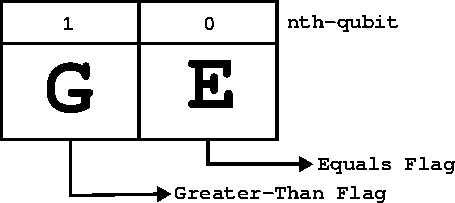
\includegraphics[scale=0.8]{images/6_Complete_System/status_reg_diagram.pdf}
    \caption{The diagram of the Status Quantum registers}
\end{figure}

\begin{listing}[!ht]
    \centering
    \begin{minted}{python3}
        from qiskit import QuantumCircuit, QuantumRegister

        op = QuantumRegister(2, name="Opcode")
        a = QuantumRegister(2, name="A")
        b = QuantumRegister(2, name="B")
        out = QuantumRegister(8, name="Out")
        stat = QuantumRegister(2, name="Status")

        qalu = QuantumCircuit(op, a, b, out, stat)
    \end{minted}
    \caption{The initialization Python code for the Quantum circuit of the Quantum ALU}
\end{listing}

After the initialization of the circuit we have to append each of the Quantum circuits that implement each of the operations
as custom Quantum gates.

To control when each of the operation will be selected accordingly to the opcode bitstring we are going to use the member
method \verb|control()| of the \verb|Gate| class. This function takes numerous parameters but we are going to use only
two of those: the \verb|num_control_qubits| and the \verb|ctrl_state| parameters. The \verb|num_control_qubits| stores
how many qubits will be used control qubits to signal the activation of the gate and the \verb|ctrl_state| parameter
annotates what is the control state of each of the control qubits. For instance, the bitstring \verb|"101"| annotates
that the least-significant and most-significant qubits will be true when in the $\ket{1}$ state and the qubit in position
1 is going to be true in the $\ket{0}$ state (inverse logic).

Using this method it is very easy to map each gate/operation to the appropriate opcode bitstring: \\\verb|ctrl_state="10"| for
the multiplication gate and \verb|ctrl_state="11"| for the comparison gate. We just have to supply the opcode register
when appending.

The addition and subtraction operations where left last because they are not that straig!ht-forward to append. These operations are
implemented by one gate that can change its mode by a control signal as an independent input. The other two operations needed
to set the \verb|num_ctrl_qubits=2| because they did not use a control signal as an input. This means that we can use one qubit
of the opcode register as an input for the Quantum Adder-Subtractor and thus we have to set \verb|num_ctrl_qubits=2| and
\verb|ctrl_state="0"| because according to the opcode table the most-significant qubit of the those operations is always in the
$\ket{0}$ state.

\begin{listing}[!ht]
    \begin{minted}{python3}
        qalu.append(addsub.control(1, ctrl_state="0"),\
            ([op[1]] + [op[0]] + a[:] + b[:] + out[:n+1]))
        qalu.append(mul.control(2, ctrl_state="10"),\
            (op[:] + a[:] + b[:] + out[:]))
        qalu.append(cmp.control(2, ctrl_state="11"),\
            (op[:] + a[:] + b[:] + out[:n+1] + stat[:]))
    \end{minted}
    \caption{Appending the custom Quantum gates of the operations to the Quantum ALU}
\end{listing}

\begin{figure}[!ht]
    \centering
    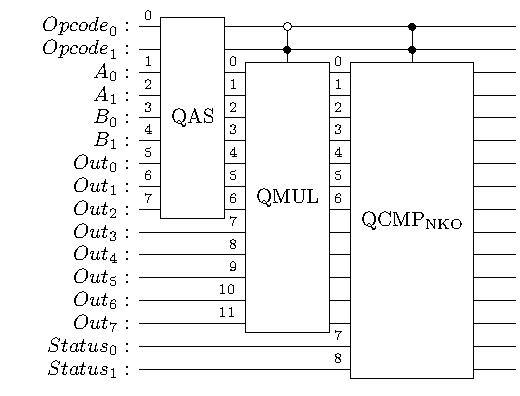
\includegraphics{images/6_Complete_System/qalu_complete.pdf}
    \caption{The Quantum circuit diagram of the Quantum ALU}
\end{figure}
\newpage
\section{Experimental Results on Simulators and Quantum Computers}
\subsection{Testing the Addition and Subtraction operations on the Aer Simulator and on a real Quantum Computer}

We will now demonstrate all of the operations of the Quantum ALU starting with addition and subtraction. Before executing any arithmetic and logic 
operation we have to initialize the Opcode register with the appropriate opcode (see Table 6.1).

Therefore, to perform an addition, the Opcode register must be initialized with the $\ket{00}$ state. For this demonstration
registers A and B are initialized with the states $\ket{11}=\ket{3}$ and $\ket{10}=\ket{2}$ respectively Listing (28):

\begin{listing}[!ht]
        \begin{minted}{python3}
            qalu.x(a[0])
            qalu.x(a[1]) # a = 11
            qalu.x(b[1]) # b = 10
        \end{minted}
        \caption{Initializing the Quantum registers A and B with the appropriate values}
        \label{ls:6_init_add}
\end{listing}

Executing the Quantum ALU circuit on an Aer simulator, the Output register arrives at the state $\ket{00000101}=\ket{5}$ which is the expected value.
In Figure (6.3) we can see this even more clearly (we omitted the five leading zeros for a clearer picture of the result):

\begin{figure}[!ht]
        \centering
        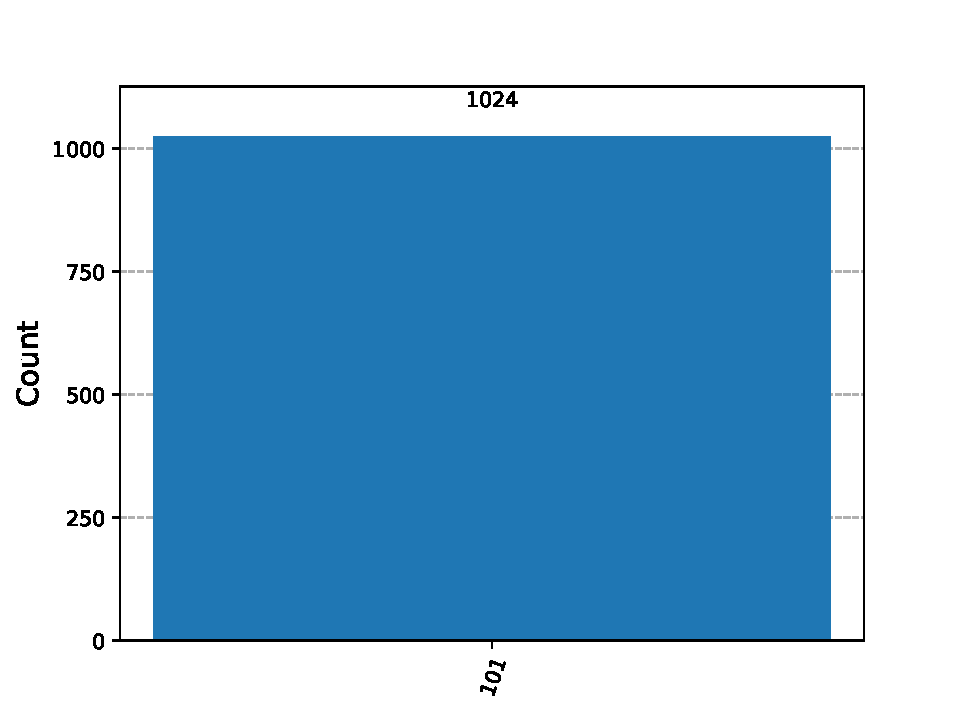
\includegraphics[scale=0.7]{images/6_Complete_System/adder_subtractor_aer_result.pdf}
        \caption{The histogram of the possible values of the Output register when the Quantum ALU performed an addition with A=3 (11) and B=2 (10) on the Aer Simulator}
\end{figure}

We shall now execute a subtraction operation with the same initial values for the A and B registers and submit a job to an IBM Quantum Computer
so that the circuit can be executed. We want to note that the expected output is $101_2$ which can be interpreted in many ways but because
the Adder-Subtractor implements a design where it performs signed and unsigned-mangitude addition and subtraction and because $A \geq B$ the
third qubit of the output register can be omitted thus the result becomes $01_2$ or just $1$ which is the expected output.

Before showing any experimental results, we would like to note that the Aer simulator and the IBM Quantum Computers execute the quantum circuits
multiple times. The Aer simulator executes them 1024 times while the IBM Quantum Computers execute them four times more, or 4096 times. Thus the
probability of the state of a specific quantum register is either obtained by the following equation:

\begin{equation}
    P(o) = \lceil \frac{c}{n}100 \rceil
\end{equation}
where $o$ is the state of the quantum register, $c$ is the \textit{count}, the number of times the specific state was the actual output, and $n$ is the total number
of executions which can be either 1024 (for the Aer simulations) or 4096 (for any IBM Quantum Computer).

In Figure (6.4) we can see multiple expected output values. Although we did not use any gate that puts any qubit in superposition, Quantum Computers
are vulnerable to noise. Noise, just like in classical computers, can cause problems like flipping a single bit's state from example; a memory cell
of a Random Access Memory module. In the case of the Quantum computer, a qubit can be flipped and give erroneous results.

\begin{figure}[!ht]
        \centering
        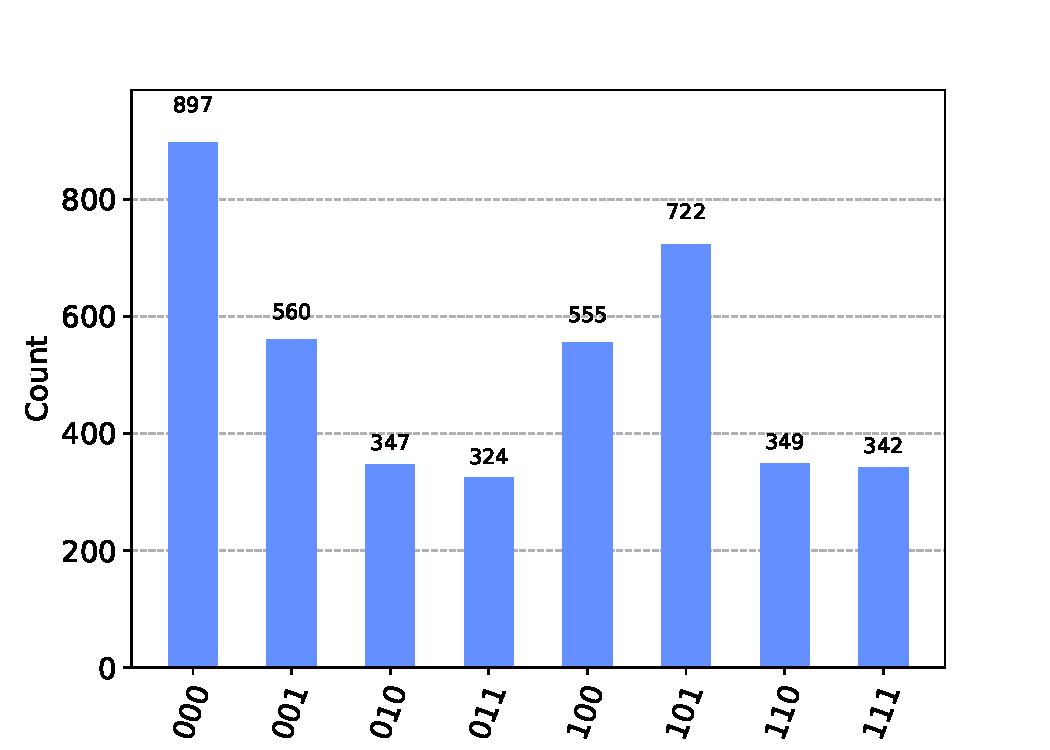
\includegraphics[scale=0.7]{images/6_Complete_System/adder_subtractor_ibmq_result.pdf}
        \caption{The histogram of the possible values of the Output register (with omitted the five leading zero'ed qubits) when the Quantum ALU performed
        an addition with A=3 (11) and B=2 (10) on the IBM Kyoto Quantum Computer}
\end{figure}

We can see that the expected value ($101_2$) has a probability of $17.64\%$ to be output'ed by the circuit.

\newpage
\subsection{Testing the Multiplication operation on the Aer Simulator and on a real Quantum Computer}
We shall demonstrate the multiplication operation with another pair of inputs. This time we shall initialize both A and B with the same value. We
arbitrarily chose $10_2$ or $2_{10}$.

Before anything else, we initialize the Opcode register with the appropriate opcode ($\ket{10}$) and then initialize the A and B registers.

\begin{listing}[!ht]
    \centering
    \begin{minted}{python3}
        qalu.x(op[1]) # op = 10
        qalu.x(a[1])
        qalu.x(b[1])
    \end{minted}
    \caption{The initialization of the Opcode, A and B Quantum registers to perform the multiplication operation}
\end{listing}

The result from the Aer simulator (see Figure (6.5))is what we expected. The result output only shows the qubits 0, 4, 6 and 7.

\begin{figure}[!ht]
    \centering
    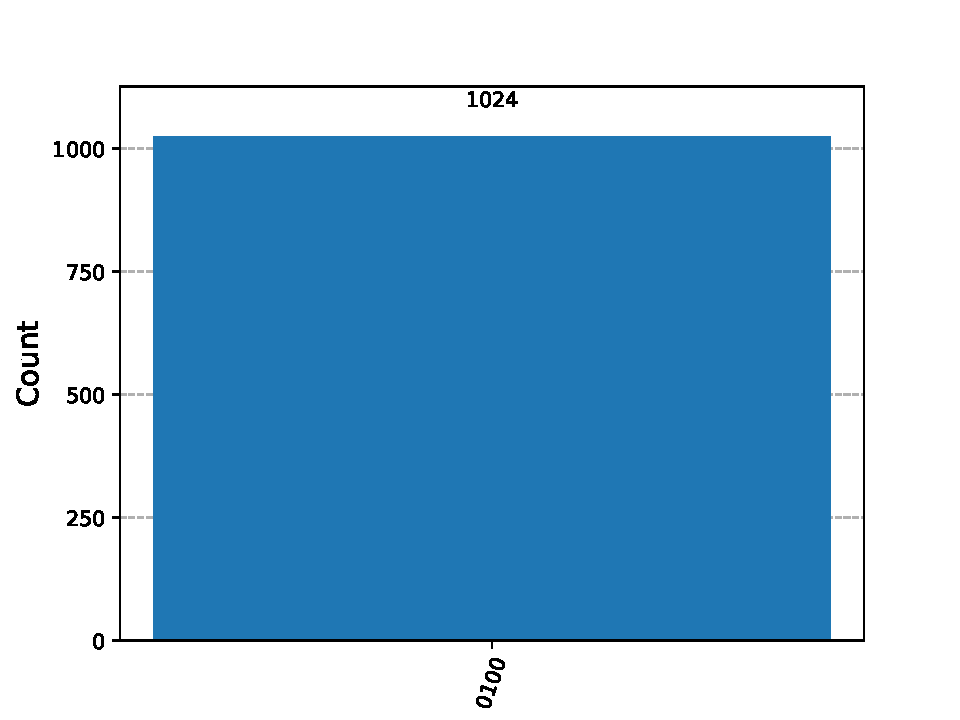
\includegraphics[scale=0.7]{images/6_Complete_System/multiplier_aer_result.pdf}
    \caption{The histogram of the possible values of the Output register when the Quantum ALU performed a multiplication with A=B=2 (10) on the Aer Simulator}
\end{figure}

Executing the same operation on a Quantum computer yields again the same behavior. We get counts of possible outputs instead of a definite answer (see Figure (6.6)).

\begin{figure}[!ht]
        \centering
        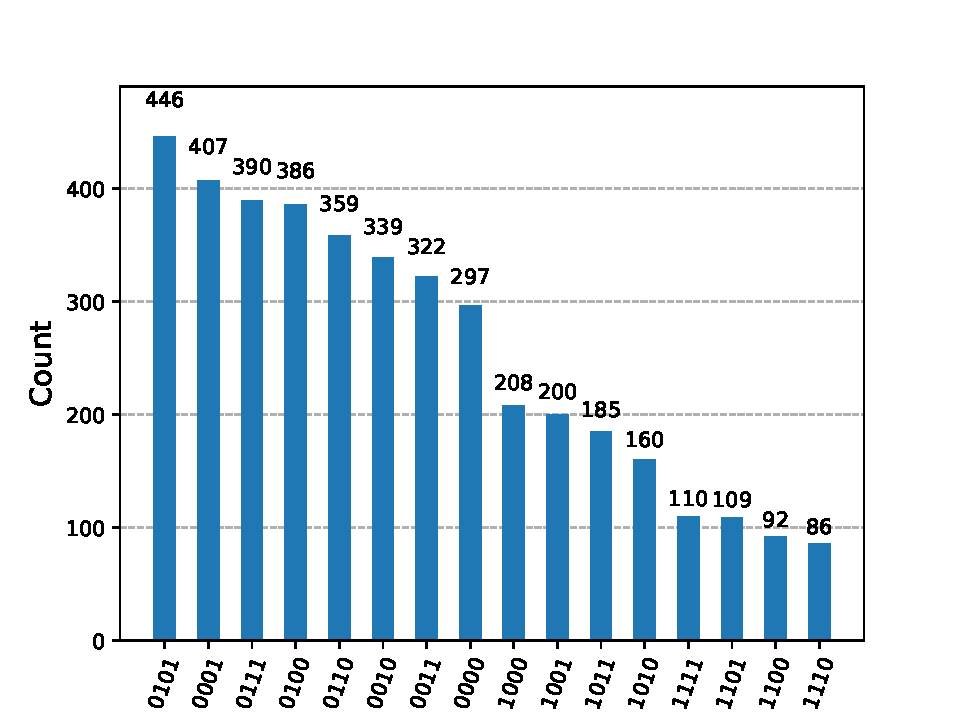
\includegraphics[scale=0.7]{images/6_Complete_System/multiplier_ibmq_result.pdf}
        \caption{The histogram of the possible values of the Output register when the Quantum ALU performed a multiplication with A=B=2 (10) on the IBM Osaka Quantum Computer}
\end{figure}

We note that the expected output ($0100_2=4_{10}$) has a $9.42\%$ probability.

\newpage
\subsection{Testing the Comparison operation on the Aer Simulator and on a real Quantum Computer}
Lastly, we executed the NKO Comparator with the two two-qubit registers inputs A and B to be again $3$ and $2$ respectively and we only measured the two qubits
of the status Quantum register. The execution of the Quantum circuit happened on the IBM Osaka Quantum Computer too. We will again contrast the real-hardware result with the
simulation results.

\begin{figure}[!ht]
    \centering
    \begin{subfigure}{0.5\textwidth}
        \centering
        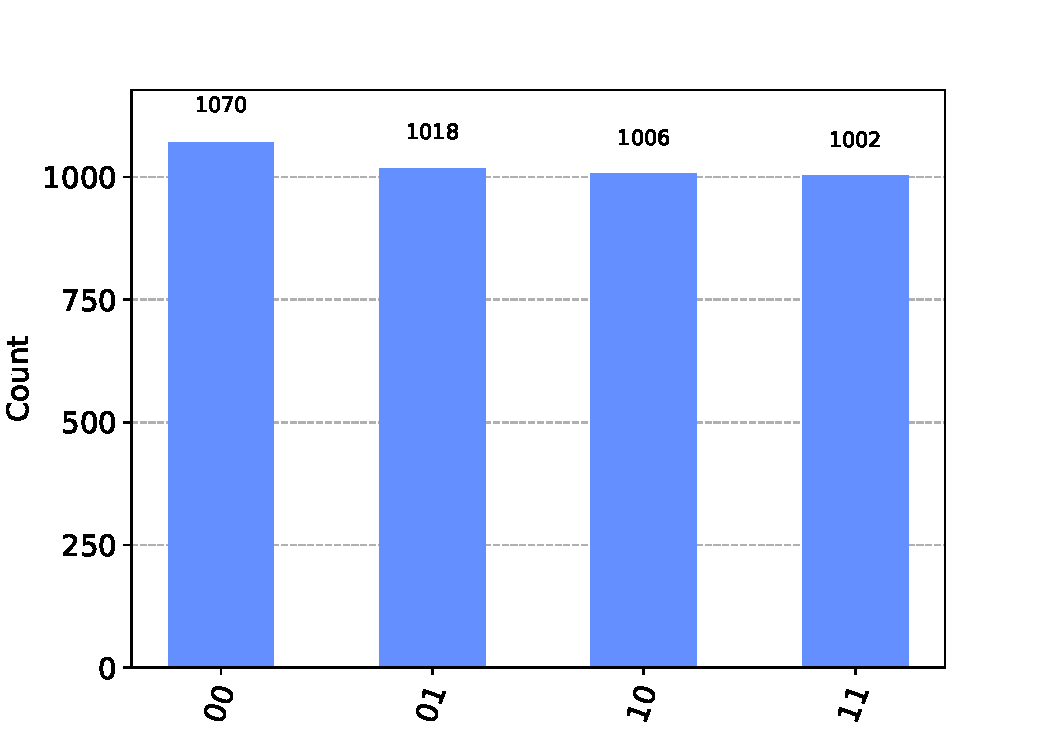
\includegraphics[scale=0.4]{images/6_Complete_System/nko_cmp_ibmq_result.pdf}
        \caption{}    
    \end{subfigure}
    \begin{subfigure}{0.5\textwidth}
        \centering
        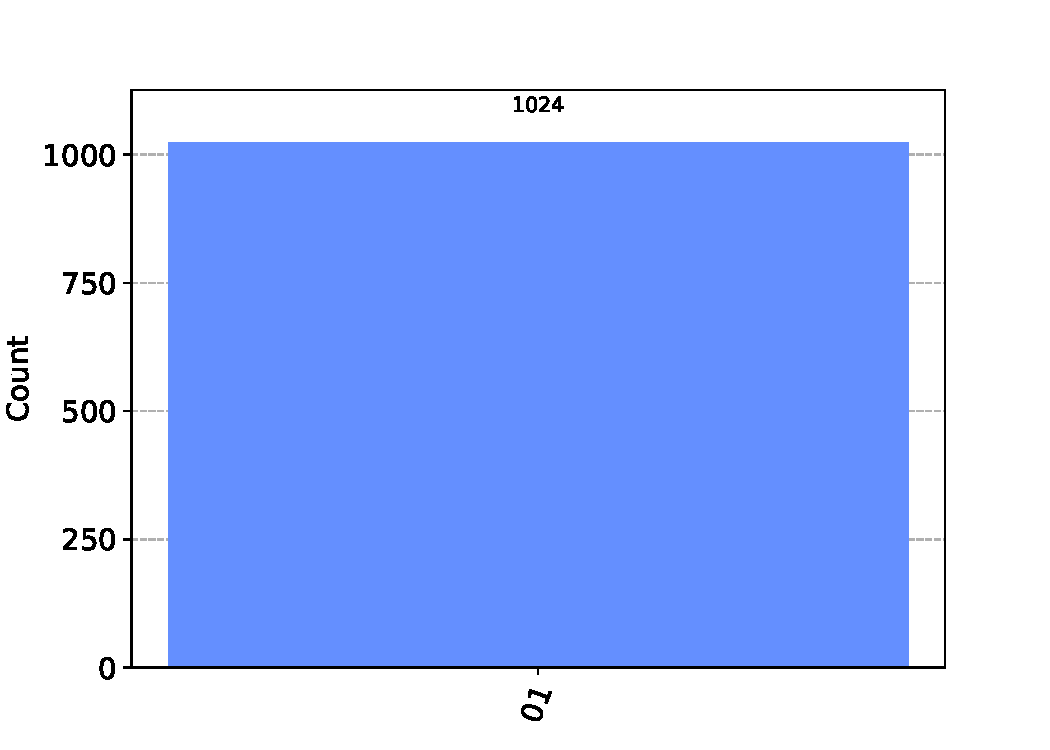
\includegraphics[scale=0.4]{images/6_Complete_System/nko_cmp_aer_result.pdf}
        \caption{}
    \end{subfigure}
    \caption{The results of the comparison operation executed on the IBM Osaka (a) and on the Aer Simulator (b)}
\end{figure}

The same story applies here, where the expected value, output'ed by the Aer Simulator, $10$ which means \say{$A\neq B\text{ and }A \geq B$}, is not the most probable output when executed
4096 times on the Quantum computer. We again compiled a table containing the probability of each output based on how many times the output occured while executing.

\begin{table}[!ht]
    \centering
    \begin{tabular}{c|c|c}
        Output Bit Sequence & Count & Probabilty ($\frac{\text{Count}}{4096}$) \\
        \hline
        $00$ & $1070$ & $26.123\%$ \\
        $01$ & $1018$ & $24.854\%$ \\
        $10$ & $1006$ & $24.561\%$ \\
        $11$ & $1002$ & $24.463\%$ \\
    \end{tabular}
    \caption{The result of probabilities of each output value of the execution of the comparison operation on the IBM Osaka}
\end{table}

We can see that each output has relatively close probability of output meaning that the Quantum computer does not give us a reliable output.
\chapter{The Complete Quantum ALU}

By gathering the previous Quantum circuits we can create the Quantum Arithmetic Logic Unit very easily. Before
we do just that we would like to take a step back and analyse how this Unit may operate.

Just like a classical ALU, the Quantum ALU operates on some general purpose registers and on a register that stores
the status of logic operations. On top of those, the Quantum ALU, may need an \textit{operation code} or \textit{opcode}
to command it to do a specific operation. We shall analyze those opcodes further.

\section{The Quantum ALU's Opcodes}

We had introduced four different Quantum circuits in the previous chapters:
\begin{enumerate}
    \item a Quantum Adder-Subtractor,
    \item a Quantum Multiplier and
    \item a Quantum Comparator
\end{enumerate}
with each Quantum circuit giving us the operations of: addition, subtraction, multiplication and magnitued comparison.
We can encode these four operations using a bitstring of length $n=2$ because $log_24=2$. The mapping of each opcode with
its corresponding operation and Quantum circuit can be seen at the table below.

\begin{table}[!ht]
    \centering
    \begin{tabular}{c|c|c}
        Opcode & Operation & Quantum circuit \\
        \hline
        \verb|00| & Addition & $QAS$ (Addition mode) \\
        \verb|01| & Subtraction & $QAS$ (Subtraction mode) \\
        \verb|10| & Multiplication & $QMUL$ \\
        \verb|11| & Magnitude Comparison & $QCMP_{NKO}$ \\
    \end{tabular}
    \caption{The Opcode table of the Quantum ALU}
\end{table}
\section{The Quantum ALU's circuit}

We will implement the Quantum ALU as any other Quantum circuit we have already presented. This Quantum circuit will have
in total sixteen qubits. The first two-qubit Quantum register is called the \textit{opcode} register and it stores the bitstring
of which operation the Quantum ALU must complete, the two two-qubit general purpose Quantum registers $A$ and $B$ is where
we store the binary encoded numbers we want to be operating, the eig!ht-qubit output Quantum register $Out$ where it is used to
store the output of each operation and lastly, the two-qubit status Quantum register $Status$ where each qubit corresponds to
a logic flag.

\begin{figure}[!ht]
    \centering
    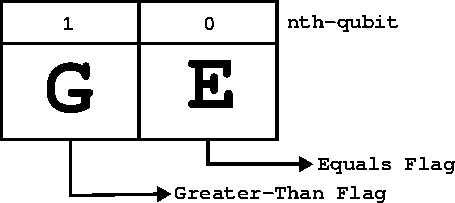
\includegraphics[scale=0.8]{images/6_Complete_System/status_reg_diagram.pdf}
    \caption{The diagram of the Status Quantum registers}
\end{figure}

\begin{listing}[!ht]
    \centering
    \begin{minted}{python3}
        from qiskit import QuantumCircuit, QuantumRegister

        op = QuantumRegister(2, name="Opcode")
        a = QuantumRegister(2, name="A")
        b = QuantumRegister(2, name="B")
        out = QuantumRegister(8, name="Out")
        stat = QuantumRegister(2, name="Status")

        qalu = QuantumCircuit(op, a, b, out, stat)
    \end{minted}
    \caption{The initialization Python code for the Quantum circuit of the Quantum ALU}
\end{listing}

After the initialization of the circuit we have to append each of the Quantum circuits that implement each of the operations
as custom Quantum gates.

To control when each of the operation will be selected accordingly to the opcode bitstring we are going to use the member
method \verb|control()| of the \verb|Gate| class. This function takes numerous parameters but we are going to use only
two of those: the \verb|num_control_qubits| and the \verb|ctrl_state| parameters. The \verb|num_control_qubits| stores
how many qubits will be used control qubits to signal the activation of the gate and the \verb|ctrl_state| parameter
annotates what is the control state of each of the control qubits. For instance, the bitstring \verb|"101"| annotates
that the least-significant and most-significant qubits will be true when in the $\ket{1}$ state and the qubit in position
1 is going to be true in the $\ket{0}$ state (inverse logic).

Using this method it is very easy to map each gate/operation to the appropriate opcode bitstring: \\\verb|ctrl_state="10"| for
the multiplication gate and \verb|ctrl_state="11"| for the comparison gate. We just have to supply the opcode register
when appending.

The addition and subtraction operations where left last because they are not that straig!ht-forward to append. These operations are
implemented by one gate that can change its mode by a control signal as an independent input. The other two operations needed
to set the \verb|num_ctrl_qubits=2| because they did not use a control signal as an input. This means that we can use one qubit
of the opcode register as an input for the Quantum Adder-Subtractor and thus we have to set \verb|num_ctrl_qubits=2| and
\verb|ctrl_state="0"| because according to the opcode table the most-significant qubit of the those operations is always in the
$\ket{0}$ state.

\begin{listing}[!ht]
    \begin{minted}{python3}
        qalu.append(addsub.control(1, ctrl_state="0"),\
            ([op[1]] + [op[0]] + a[:] + b[:] + out[:n+1]))
        qalu.append(mul.control(2, ctrl_state="10"),\
            (op[:] + a[:] + b[:] + out[:]))
        qalu.append(cmp.control(2, ctrl_state="11"),\
            (op[:] + a[:] + b[:] + out[:n+1] + stat[:]))
    \end{minted}
    \caption{Appending the custom Quantum gates of the operations to the Quantum ALU}
\end{listing}

\begin{figure}[!ht]
    \centering
    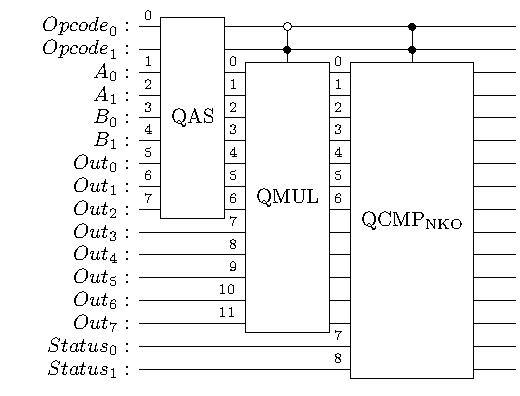
\includegraphics{images/6_Complete_System/qalu_complete.pdf}
    \caption{The Quantum circuit diagram of the Quantum ALU}
\end{figure}
\newpage
\section{Experimental Results on Simulators and Quantum Computers}
\subsection{Testing the Addition and Subtraction operations on the Aer Simulator and on a real Quantum Computer}

We will now demonstrate all of the operations of the Quantum ALU starting with addition and subtraction. Before executing any arithmetic and logic 
operation we have to initialize the Opcode register with the appropriate opcode (see Table 6.1).

Therefore, to perform an addition, the Opcode register must be initialized with the $\ket{00}$ state. For this demonstration
registers A and B are initialized with the states $\ket{11}=\ket{3}$ and $\ket{10}=\ket{2}$ respectively Listing (28):

\begin{listing}[!ht]
        \begin{minted}{python3}
            qalu.x(a[0])
            qalu.x(a[1]) # a = 11
            qalu.x(b[1]) # b = 10
        \end{minted}
        \caption{Initializing the Quantum registers A and B with the appropriate values}
        \label{ls:6_init_add}
\end{listing}

Executing the Quantum ALU circuit on an Aer simulator, the Output register arrives at the state $\ket{00000101}=\ket{5}$ which is the expected value.
In Figure (6.3) we can see this even more clearly (we omitted the five leading zeros for a clearer picture of the result):

\begin{figure}[!ht]
        \centering
        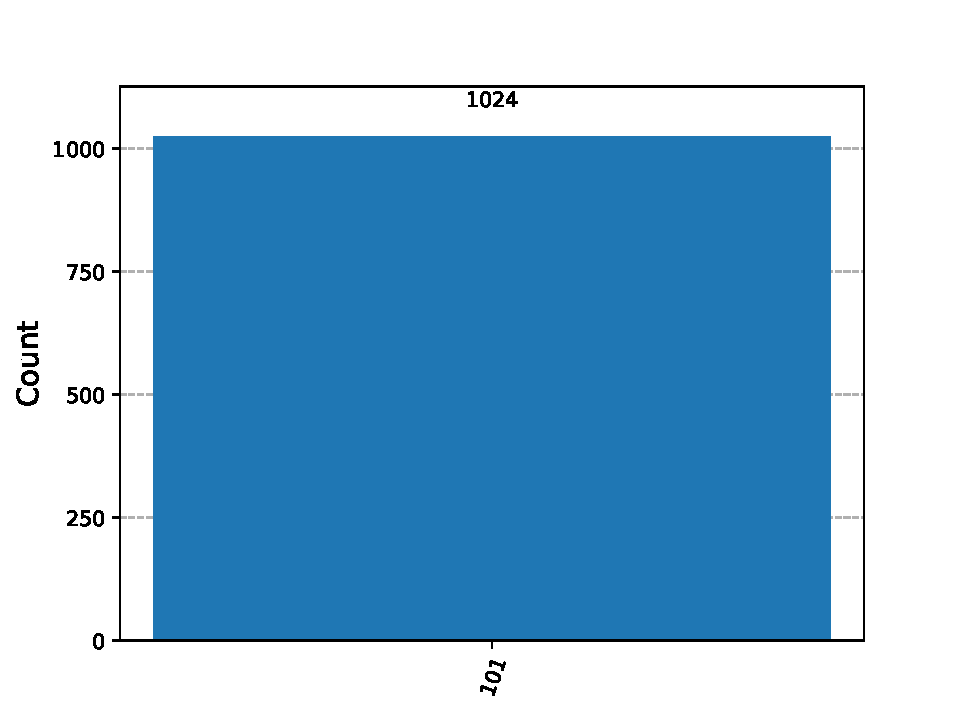
\includegraphics[scale=0.7]{images/6_Complete_System/adder_subtractor_aer_result.pdf}
        \caption{The histogram of the possible values of the Output register when the Quantum ALU performed an addition with A=3 (11) and B=2 (10) on the Aer Simulator}
\end{figure}

We shall now execute a subtraction operation with the same initial values for the A and B registers and submit a job to an IBM Quantum Computer
so that the circuit can be executed. We want to note that the expected output is $101_2$ which can be interpreted in many ways but because
the Adder-Subtractor implements a design where it performs signed and unsigned-mangitude addition and subtraction and because $A \geq B$ the
third qubit of the output register can be omitted thus the result becomes $01_2$ or just $1$ which is the expected output.

Before showing any experimental results, we would like to note that the Aer simulator and the IBM Quantum Computers execute the quantum circuits
multiple times. The Aer simulator executes them 1024 times while the IBM Quantum Computers execute them four times more, or 4096 times. Thus the
probability of the state of a specific quantum register is either obtained by the following equation:

\begin{equation}
    P(o) = \lceil \frac{c}{n}100 \rceil
\end{equation}
where $o$ is the state of the quantum register, $c$ is the \textit{count}, the number of times the specific state was the actual output, and $n$ is the total number
of executions which can be either 1024 (for the Aer simulations) or 4096 (for any IBM Quantum Computer).

In Figure (6.4) we can see multiple expected output values. Although we did not use any gate that puts any qubit in superposition, Quantum Computers
are vulnerable to noise. Noise, just like in classical computers, can cause problems like flipping a single bit's state from example; a memory cell
of a Random Access Memory module. In the case of the Quantum computer, a qubit can be flipped and give erroneous results.

\begin{figure}[!ht]
        \centering
        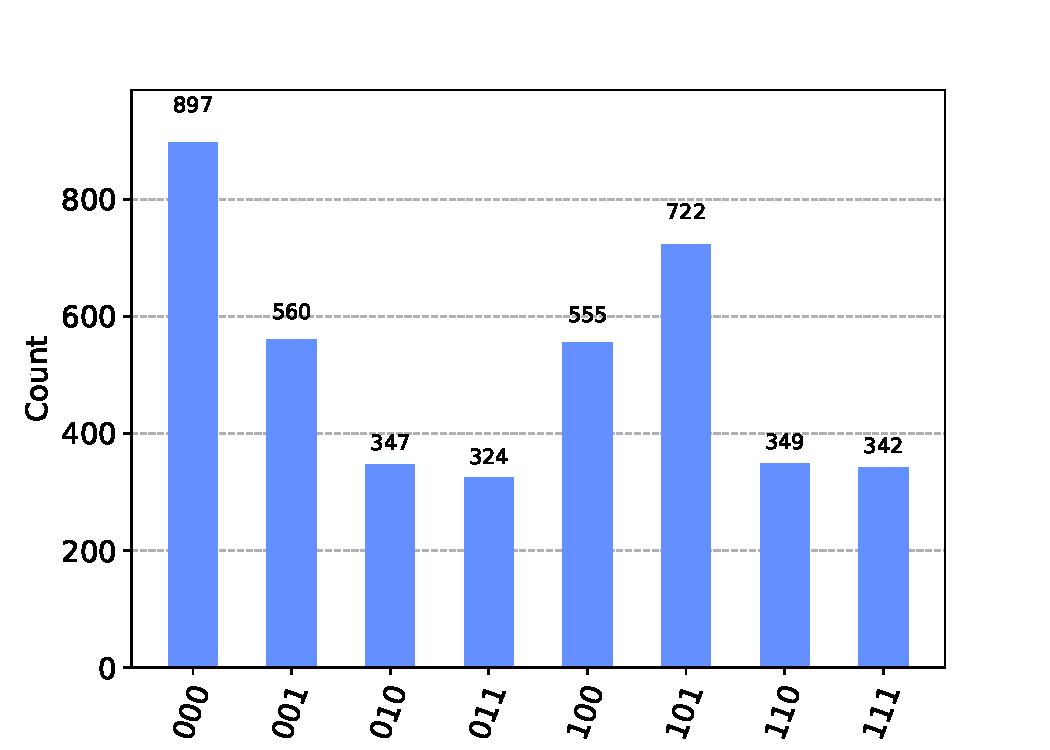
\includegraphics[scale=0.7]{images/6_Complete_System/adder_subtractor_ibmq_result.pdf}
        \caption{The histogram of the possible values of the Output register (with omitted the five leading zero'ed qubits) when the Quantum ALU performed
        an addition with A=3 (11) and B=2 (10) on the IBM Kyoto Quantum Computer}
\end{figure}

We can see that the expected value ($101_2$) has a probability of $17.64\%$ to be output'ed by the circuit.

\newpage
\subsection{Testing the Multiplication operation on the Aer Simulator and on a real Quantum Computer}
We shall demonstrate the multiplication operation with another pair of inputs. This time we shall initialize both A and B with the same value. We
arbitrarily chose $10_2$ or $2_{10}$.

Before anything else, we initialize the Opcode register with the appropriate opcode ($\ket{10}$) and then initialize the A and B registers.

\begin{listing}[!ht]
    \centering
    \begin{minted}{python3}
        qalu.x(op[1]) # op = 10
        qalu.x(a[1])
        qalu.x(b[1])
    \end{minted}
    \caption{The initialization of the Opcode, A and B Quantum registers to perform the multiplication operation}
\end{listing}

The result from the Aer simulator (see Figure (6.5))is what we expected. The result output only shows the qubits 0, 4, 6 and 7.

\begin{figure}[!ht]
    \centering
    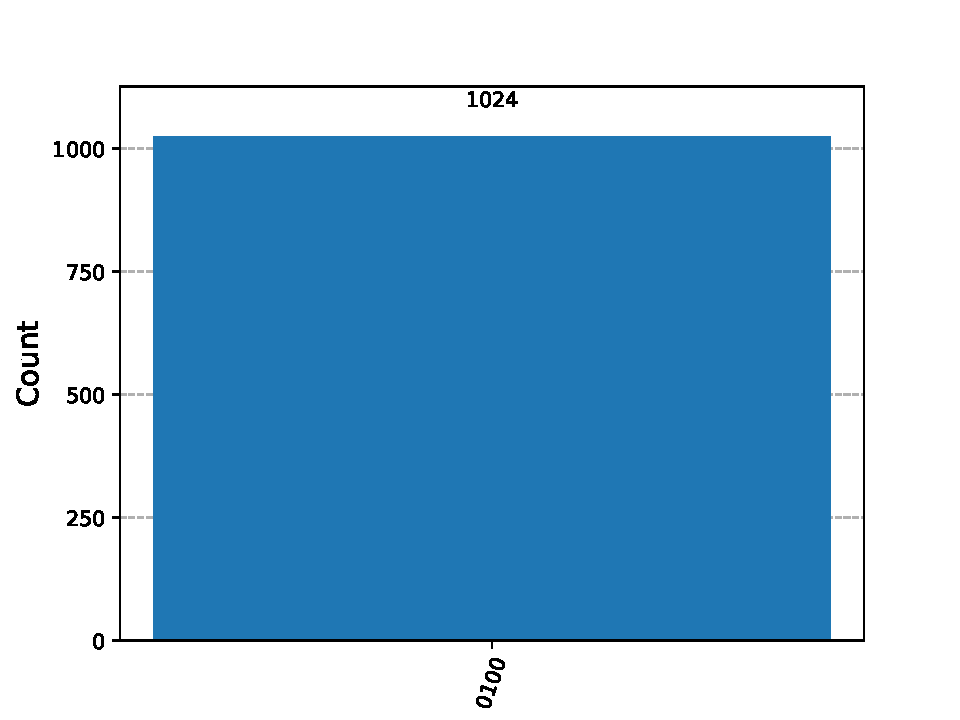
\includegraphics[scale=0.7]{images/6_Complete_System/multiplier_aer_result.pdf}
    \caption{The histogram of the possible values of the Output register when the Quantum ALU performed a multiplication with A=B=2 (10) on the Aer Simulator}
\end{figure}

Executing the same operation on a Quantum computer yields again the same behavior. We get counts of possible outputs instead of a definite answer (see Figure (6.6)).

\begin{figure}[!ht]
        \centering
        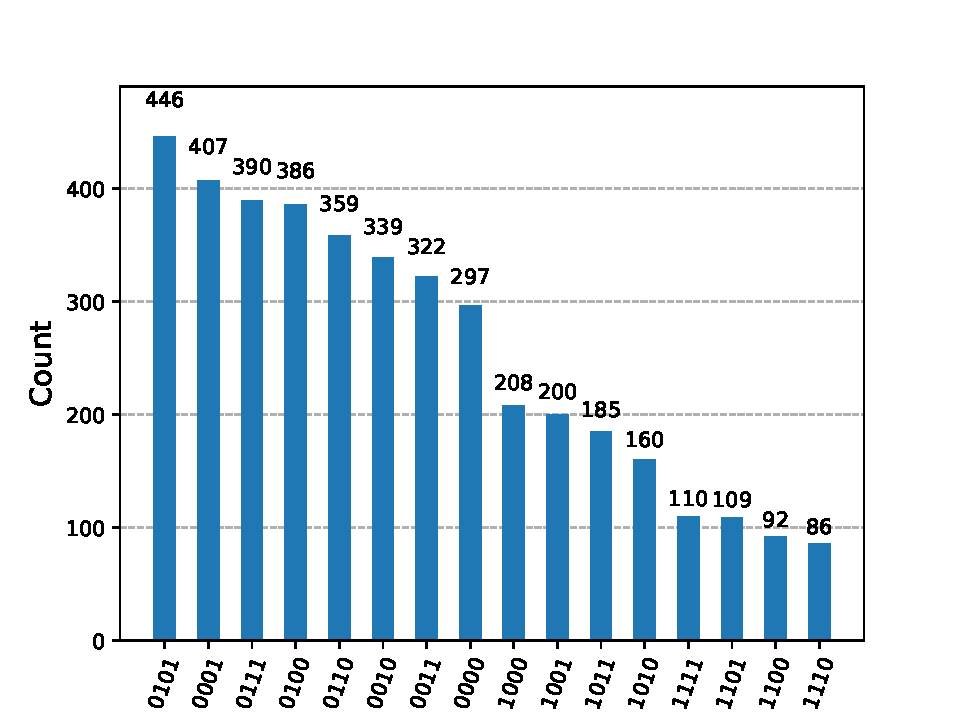
\includegraphics[scale=0.7]{images/6_Complete_System/multiplier_ibmq_result.pdf}
        \caption{The histogram of the possible values of the Output register when the Quantum ALU performed a multiplication with A=B=2 (10) on the IBM Osaka Quantum Computer}
\end{figure}

We note that the expected output ($0100_2=4_{10}$) has a $9.42\%$ probability.

\newpage
\subsection{Testing the Comparison operation on the Aer Simulator and on a real Quantum Computer}
Lastly, we executed the NKO Comparator with the two two-qubit registers inputs A and B to be again $3$ and $2$ respectively and we only measured the two qubits
of the status Quantum register. The execution of the Quantum circuit happened on the IBM Osaka Quantum Computer too. We will again contrast the real-hardware result with the
simulation results.

\begin{figure}[!ht]
    \centering
    \begin{subfigure}{0.5\textwidth}
        \centering
        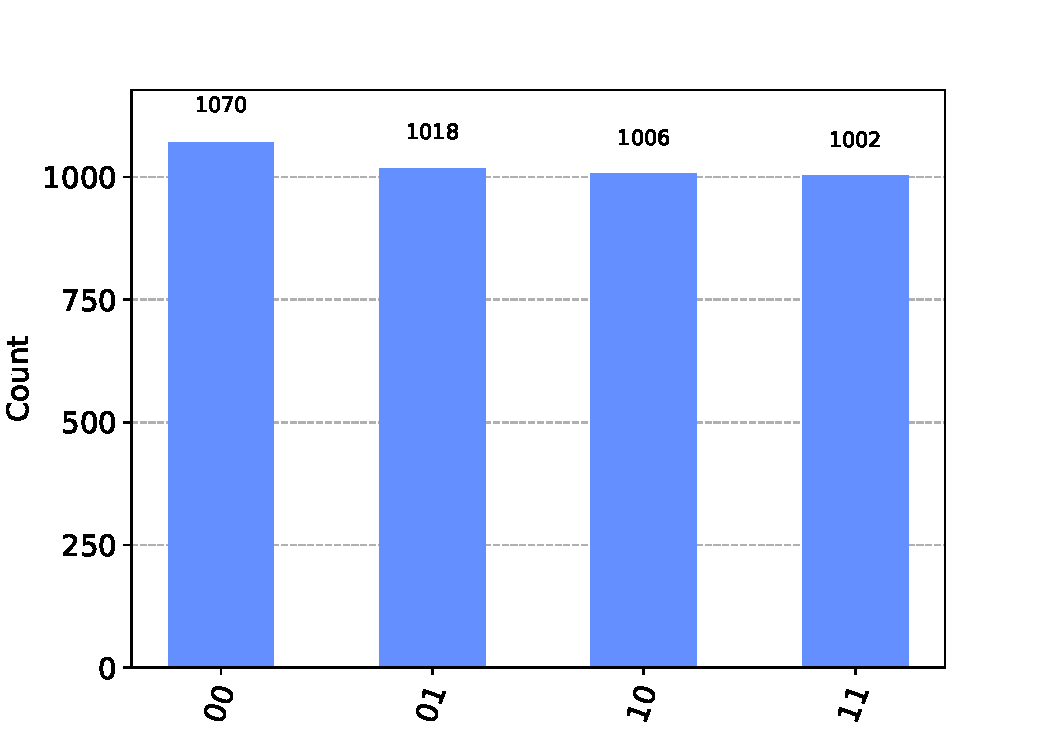
\includegraphics[scale=0.4]{images/6_Complete_System/nko_cmp_ibmq_result.pdf}
        \caption{}    
    \end{subfigure}
    \begin{subfigure}{0.5\textwidth}
        \centering
        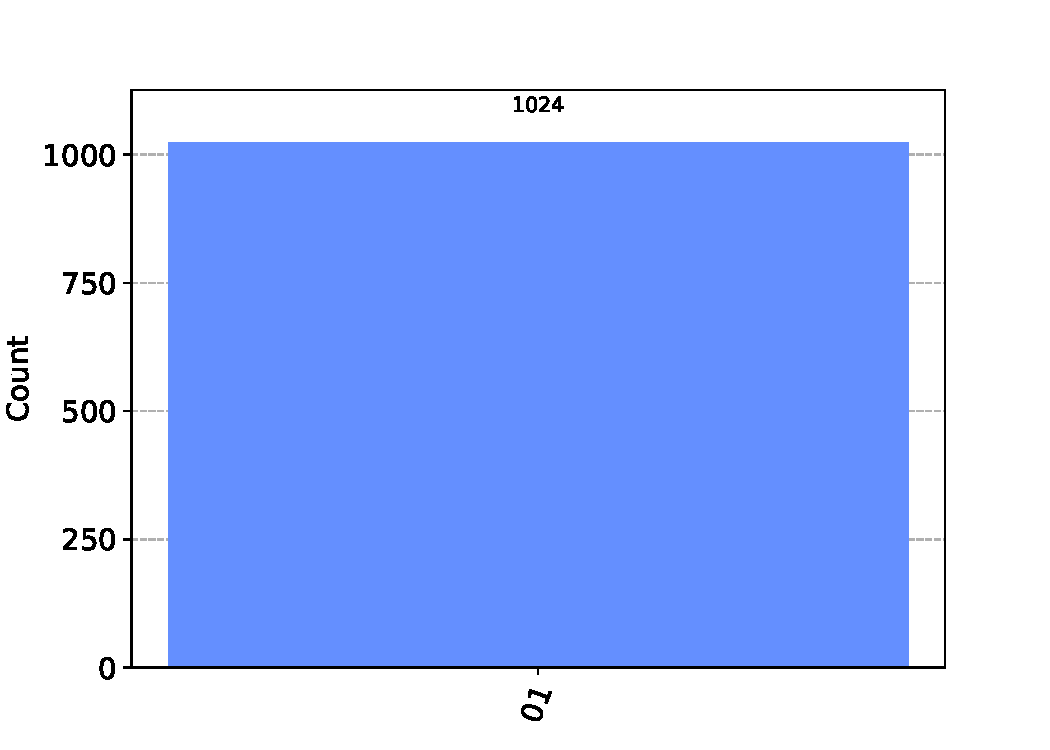
\includegraphics[scale=0.4]{images/6_Complete_System/nko_cmp_aer_result.pdf}
        \caption{}
    \end{subfigure}
    \caption{The results of the comparison operation executed on the IBM Osaka (a) and on the Aer Simulator (b)}
\end{figure}

The same story applies here, where the expected value, output'ed by the Aer Simulator, $10$ which means \say{$A\neq B\text{ and }A \geq B$}, is not the most probable output when executed
4096 times on the Quantum computer. We again compiled a table containing the probability of each output based on how many times the output occured while executing.

\begin{table}[!ht]
    \centering
    \begin{tabular}{c|c|c}
        Output Bit Sequence & Count & Probabilty ($\frac{\text{Count}}{4096}$) \\
        \hline
        $00$ & $1070$ & $26.123\%$ \\
        $01$ & $1018$ & $24.854\%$ \\
        $10$ & $1006$ & $24.561\%$ \\
        $11$ & $1002$ & $24.463\%$ \\
    \end{tabular}
    \caption{The result of probabilities of each output value of the execution of the comparison operation on the IBM Osaka}
\end{table}

We can see that each output has relatively close probability of output meaning that the Quantum computer does not give us a reliable output.
\chapter{The Complete Quantum ALU}

By gathering the previous Quantum circuits we can create the Quantum Arithmetic Logic Unit very easily. Before
we do just that we would like to take a step back and analyse how this Unit may operate.

Just like a classical ALU, the Quantum ALU operates on some general purpose registers and on a register that stores
the status of logic operations. On top of those, the Quantum ALU, may need an \textit{operation code} or \textit{opcode}
to command it to do a specific operation. We shall analyze those opcodes further.

\section{The Quantum ALU's Opcodes}

We had introduced four different Quantum circuits in the previous chapters:
\begin{enumerate}
    \item a Quantum Adder-Subtractor,
    \item a Quantum Multiplier and
    \item a Quantum Comparator
\end{enumerate}
with each Quantum circuit giving us the operations of: addition, subtraction, multiplication and magnitued comparison.
We can encode these four operations using a bitstring of length $n=2$ because $log_24=2$. The mapping of each opcode with
its corresponding operation and Quantum circuit can be seen at the table below.

\begin{table}[!ht]
    \centering
    \begin{tabular}{c|c|c}
        Opcode & Operation & Quantum circuit \\
        \hline
        \verb|00| & Addition & $QAS$ (Addition mode) \\
        \verb|01| & Subtraction & $QAS$ (Subtraction mode) \\
        \verb|10| & Multiplication & $QMUL$ \\
        \verb|11| & Magnitude Comparison & $QCMP_{NKO}$ \\
    \end{tabular}
    \caption{The Opcode table of the Quantum ALU}
\end{table}
\section{The Quantum ALU's circuit}

We will implement the Quantum ALU as any other Quantum circuit we have already presented. This Quantum circuit will have
in total sixteen qubits. The first two-qubit Quantum register is called the \textit{opcode} register and it stores the bitstring
of which operation the Quantum ALU must complete, the two two-qubit general purpose Quantum registers $A$ and $B$ is where
we store the binary encoded numbers we want to be operating, the eig!ht-qubit output Quantum register $Out$ where it is used to
store the output of each operation and lastly, the two-qubit status Quantum register $Status$ where each qubit corresponds to
a logic flag.

\begin{figure}[!ht]
    \centering
    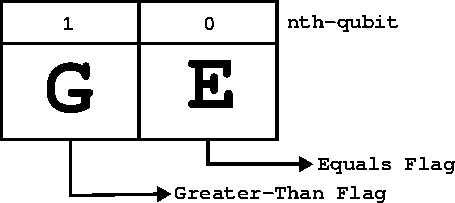
\includegraphics[scale=0.8]{images/6_Complete_System/status_reg_diagram.pdf}
    \caption{The diagram of the Status Quantum registers}
\end{figure}

\begin{listing}[!ht]
    \centering
    \begin{minted}{python3}
        from qiskit import QuantumCircuit, QuantumRegister

        op = QuantumRegister(2, name="Opcode")
        a = QuantumRegister(2, name="A")
        b = QuantumRegister(2, name="B")
        out = QuantumRegister(8, name="Out")
        stat = QuantumRegister(2, name="Status")

        qalu = QuantumCircuit(op, a, b, out, stat)
    \end{minted}
    \caption{The initialization Python code for the Quantum circuit of the Quantum ALU}
\end{listing}

After the initialization of the circuit we have to append each of the Quantum circuits that implement each of the operations
as custom Quantum gates.

To control when each of the operation will be selected accordingly to the opcode bitstring we are going to use the member
method \verb|control()| of the \verb|Gate| class. This function takes numerous parameters but we are going to use only
two of those: the \verb|num_control_qubits| and the \verb|ctrl_state| parameters. The \verb|num_control_qubits| stores
how many qubits will be used control qubits to signal the activation of the gate and the \verb|ctrl_state| parameter
annotates what is the control state of each of the control qubits. For instance, the bitstring \verb|"101"| annotates
that the least-significant and most-significant qubits will be true when in the $\ket{1}$ state and the qubit in position
1 is going to be true in the $\ket{0}$ state (inverse logic).

Using this method it is very easy to map each gate/operation to the appropriate opcode bitstring: \\\verb|ctrl_state="10"| for
the multiplication gate and \verb|ctrl_state="11"| for the comparison gate. We just have to supply the opcode register
when appending.

The addition and subtraction operations where left last because they are not that straig!ht-forward to append. These operations are
implemented by one gate that can change its mode by a control signal as an independent input. The other two operations needed
to set the \verb|num_ctrl_qubits=2| because they did not use a control signal as an input. This means that we can use one qubit
of the opcode register as an input for the Quantum Adder-Subtractor and thus we have to set \verb|num_ctrl_qubits=2| and
\verb|ctrl_state="0"| because according to the opcode table the most-significant qubit of the those operations is always in the
$\ket{0}$ state.

\begin{listing}[!ht]
    \begin{minted}{python3}
        qalu.append(addsub.control(1, ctrl_state="0"),\
            ([op[1]] + [op[0]] + a[:] + b[:] + out[:n+1]))
        qalu.append(mul.control(2, ctrl_state="10"),\
            (op[:] + a[:] + b[:] + out[:]))
        qalu.append(cmp.control(2, ctrl_state="11"),\
            (op[:] + a[:] + b[:] + out[:n+1] + stat[:]))
    \end{minted}
    \caption{Appending the custom Quantum gates of the operations to the Quantum ALU}
\end{listing}

\begin{figure}[!ht]
    \centering
    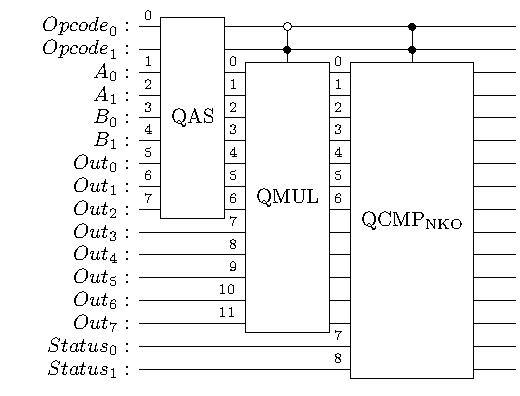
\includegraphics{images/6_Complete_System/qalu_complete.pdf}
    \caption{The Quantum circuit diagram of the Quantum ALU}
\end{figure}
\newpage
\section{Experimental Results on Simulators and Quantum Computers}
\subsection{Testing the Addition and Subtraction operations on the Aer Simulator and on a real Quantum Computer}

We will now demonstrate all of the operations of the Quantum ALU starting with addition and subtraction. Before executing any arithmetic and logic 
operation we have to initialize the Opcode register with the appropriate opcode (see Table 6.1).

Therefore, to perform an addition, the Opcode register must be initialized with the $\ket{00}$ state. For this demonstration
registers A and B are initialized with the states $\ket{11}=\ket{3}$ and $\ket{10}=\ket{2}$ respectively Listing (28):

\begin{listing}[!ht]
        \begin{minted}{python3}
            qalu.x(a[0])
            qalu.x(a[1]) # a = 11
            qalu.x(b[1]) # b = 10
        \end{minted}
        \caption{Initializing the Quantum registers A and B with the appropriate values}
        \label{ls:6_init_add}
\end{listing}

Executing the Quantum ALU circuit on an Aer simulator, the Output register arrives at the state $\ket{00000101}=\ket{5}$ which is the expected value.
In Figure (6.3) we can see this even more clearly (we omitted the five leading zeros for a clearer picture of the result):

\begin{figure}[!ht]
        \centering
        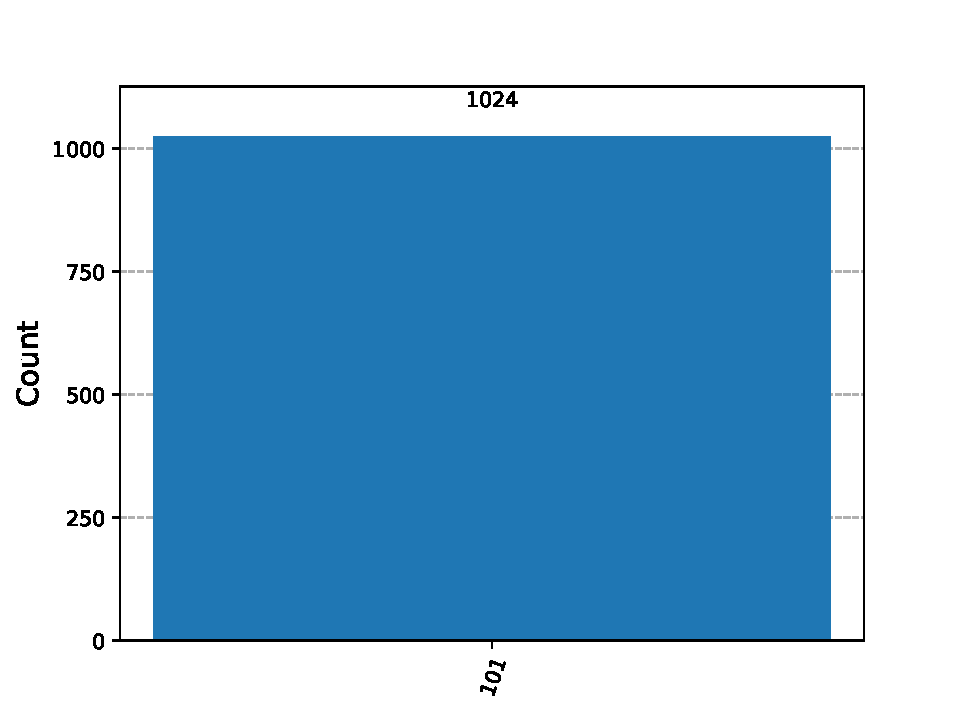
\includegraphics[scale=0.7]{images/6_Complete_System/adder_subtractor_aer_result.pdf}
        \caption{The histogram of the possible values of the Output register when the Quantum ALU performed an addition with A=3 (11) and B=2 (10) on the Aer Simulator}
\end{figure}

We shall now execute a subtraction operation with the same initial values for the A and B registers and submit a job to an IBM Quantum Computer
so that the circuit can be executed. We want to note that the expected output is $101_2$ which can be interpreted in many ways but because
the Adder-Subtractor implements a design where it performs signed and unsigned-mangitude addition and subtraction and because $A \geq B$ the
third qubit of the output register can be omitted thus the result becomes $01_2$ or just $1$ which is the expected output.

Before showing any experimental results, we would like to note that the Aer simulator and the IBM Quantum Computers execute the quantum circuits
multiple times. The Aer simulator executes them 1024 times while the IBM Quantum Computers execute them four times more, or 4096 times. Thus the
probability of the state of a specific quantum register is either obtained by the following equation:

\begin{equation}
    P(o) = \lceil \frac{c}{n}100 \rceil
\end{equation}
where $o$ is the state of the quantum register, $c$ is the \textit{count}, the number of times the specific state was the actual output, and $n$ is the total number
of executions which can be either 1024 (for the Aer simulations) or 4096 (for any IBM Quantum Computer).

In Figure (6.4) we can see multiple expected output values. Although we did not use any gate that puts any qubit in superposition, Quantum Computers
are vulnerable to noise. Noise, just like in classical computers, can cause problems like flipping a single bit's state from example; a memory cell
of a Random Access Memory module. In the case of the Quantum computer, a qubit can be flipped and give erroneous results.

\begin{figure}[!ht]
        \centering
        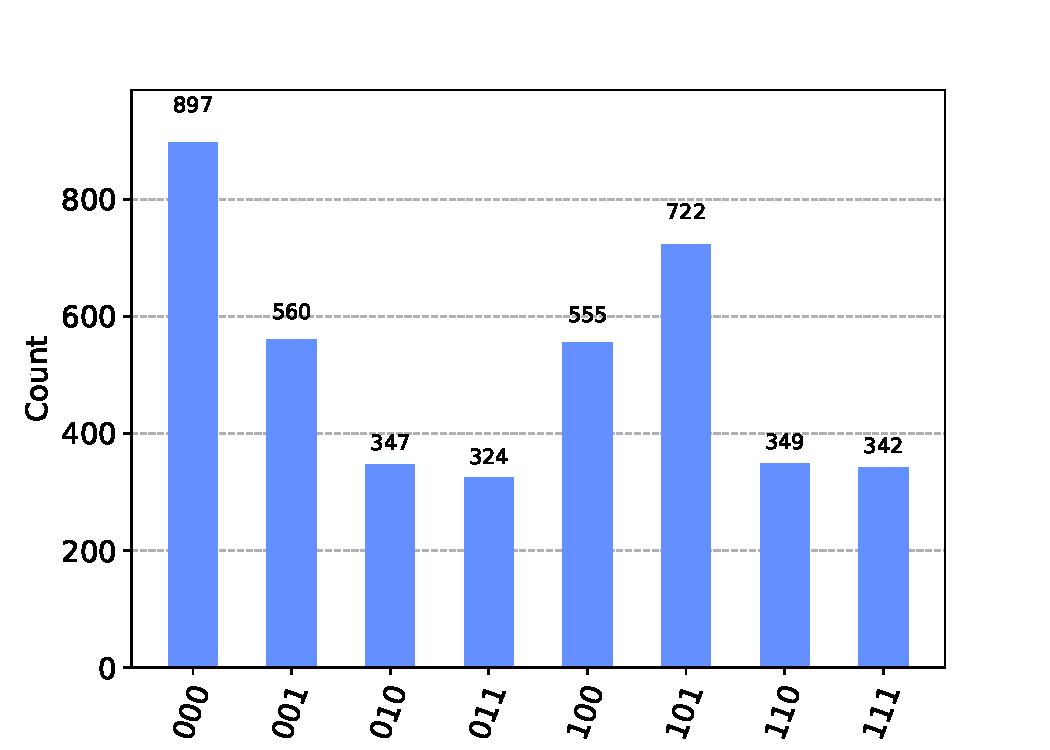
\includegraphics[scale=0.7]{images/6_Complete_System/adder_subtractor_ibmq_result.pdf}
        \caption{The histogram of the possible values of the Output register (with omitted the five leading zero'ed qubits) when the Quantum ALU performed
        an addition with A=3 (11) and B=2 (10) on the IBM Kyoto Quantum Computer}
\end{figure}

We can see that the expected value ($101_2$) has a probability of $17.64\%$ to be output'ed by the circuit.

\newpage
\subsection{Testing the Multiplication operation on the Aer Simulator and on a real Quantum Computer}
We shall demonstrate the multiplication operation with another pair of inputs. This time we shall initialize both A and B with the same value. We
arbitrarily chose $10_2$ or $2_{10}$.

Before anything else, we initialize the Opcode register with the appropriate opcode ($\ket{10}$) and then initialize the A and B registers.

\begin{listing}[!ht]
    \centering
    \begin{minted}{python3}
        qalu.x(op[1]) # op = 10
        qalu.x(a[1])
        qalu.x(b[1])
    \end{minted}
    \caption{The initialization of the Opcode, A and B Quantum registers to perform the multiplication operation}
\end{listing}

The result from the Aer simulator (see Figure (6.5))is what we expected. The result output only shows the qubits 0, 4, 6 and 7.

\begin{figure}[!ht]
    \centering
    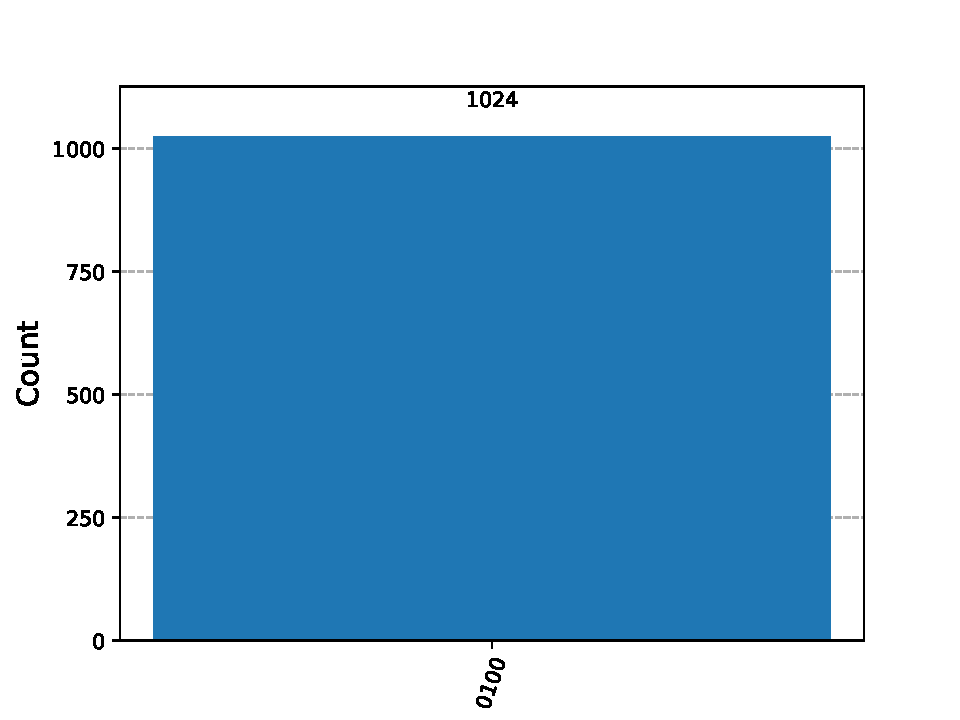
\includegraphics[scale=0.7]{images/6_Complete_System/multiplier_aer_result.pdf}
    \caption{The histogram of the possible values of the Output register when the Quantum ALU performed a multiplication with A=B=2 (10) on the Aer Simulator}
\end{figure}

Executing the same operation on a Quantum computer yields again the same behavior. We get counts of possible outputs instead of a definite answer (see Figure (6.6)).

\begin{figure}[!ht]
        \centering
        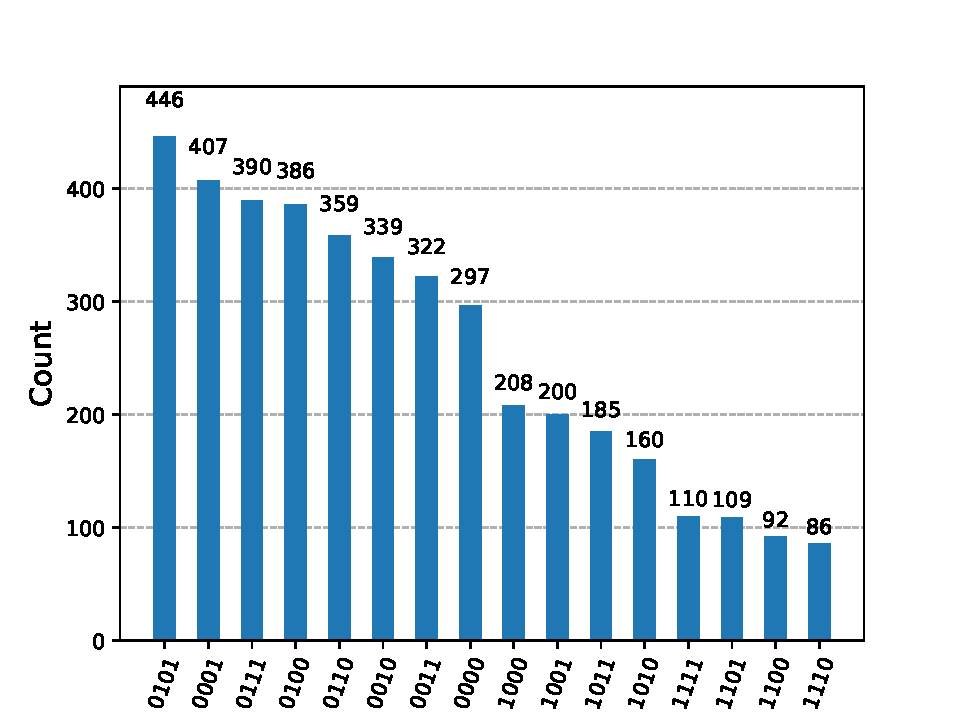
\includegraphics[scale=0.7]{images/6_Complete_System/multiplier_ibmq_result.pdf}
        \caption{The histogram of the possible values of the Output register when the Quantum ALU performed a multiplication with A=B=2 (10) on the IBM Osaka Quantum Computer}
\end{figure}

We note that the expected output ($0100_2=4_{10}$) has a $9.42\%$ probability.

\newpage
\subsection{Testing the Comparison operation on the Aer Simulator and on a real Quantum Computer}
Lastly, we executed the NKO Comparator with the two two-qubit registers inputs A and B to be again $3$ and $2$ respectively and we only measured the two qubits
of the status Quantum register. The execution of the Quantum circuit happened on the IBM Osaka Quantum Computer too. We will again contrast the real-hardware result with the
simulation results.

\begin{figure}[!ht]
    \centering
    \begin{subfigure}{0.5\textwidth}
        \centering
        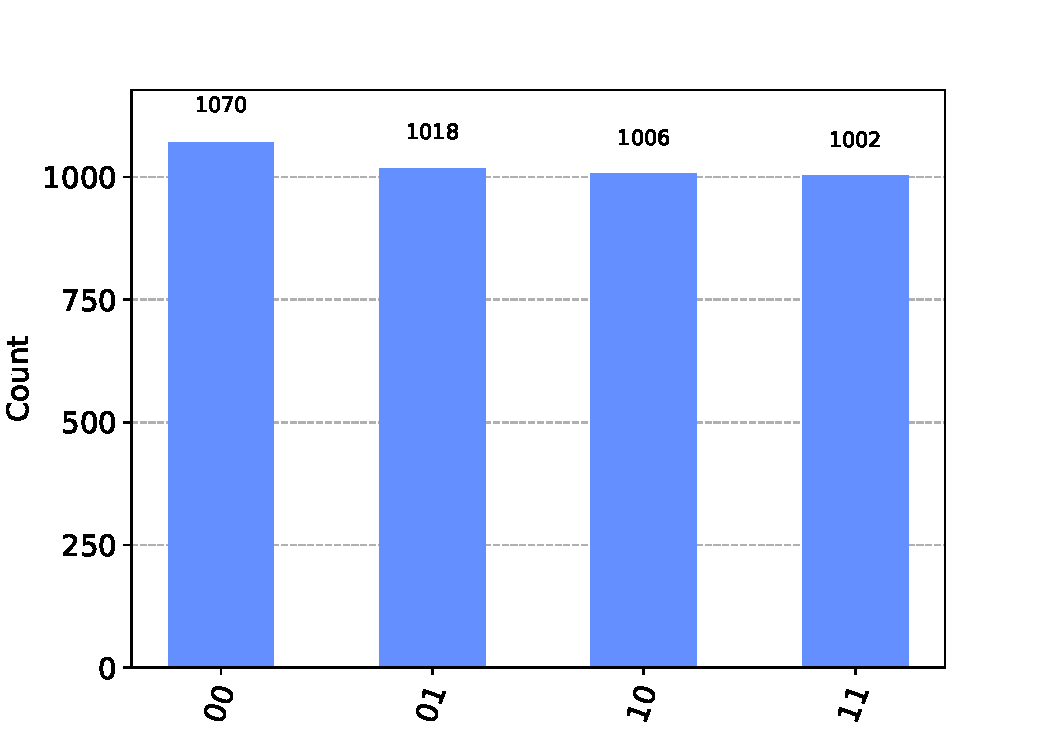
\includegraphics[scale=0.4]{images/6_Complete_System/nko_cmp_ibmq_result.pdf}
        \caption{}    
    \end{subfigure}
    \begin{subfigure}{0.5\textwidth}
        \centering
        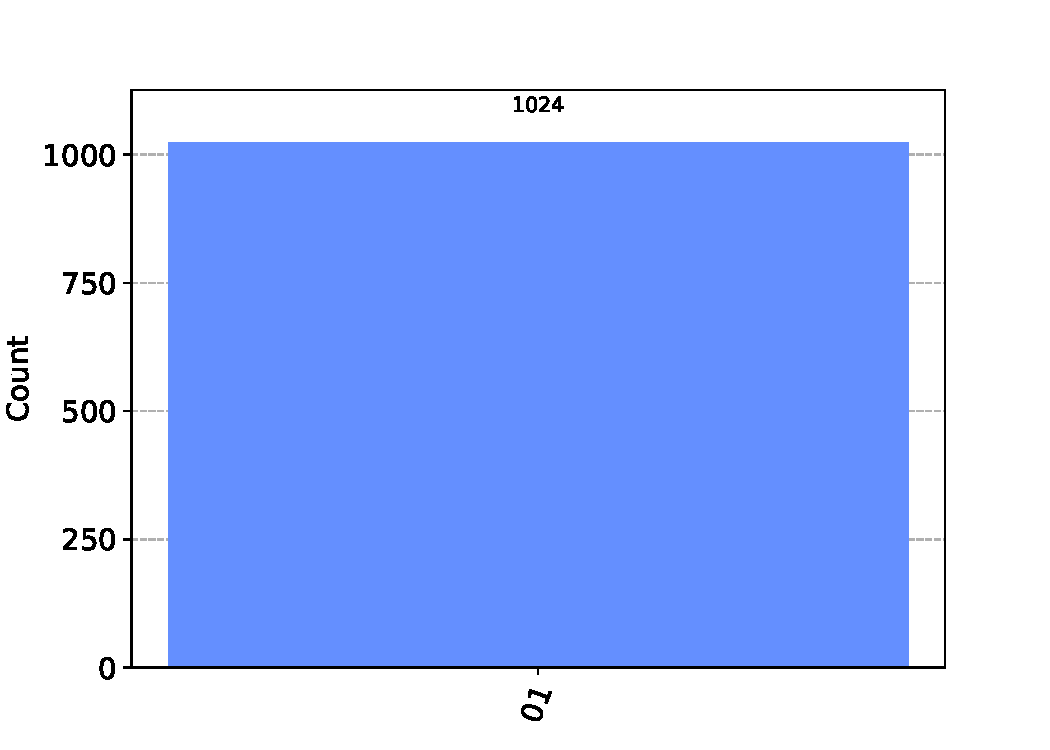
\includegraphics[scale=0.4]{images/6_Complete_System/nko_cmp_aer_result.pdf}
        \caption{}
    \end{subfigure}
    \caption{The results of the comparison operation executed on the IBM Osaka (a) and on the Aer Simulator (b)}
\end{figure}

The same story applies here, where the expected value, output'ed by the Aer Simulator, $10$ which means \say{$A\neq B\text{ and }A \geq B$}, is not the most probable output when executed
4096 times on the Quantum computer. We again compiled a table containing the probability of each output based on how many times the output occured while executing.

\begin{table}[!ht]
    \centering
    \begin{tabular}{c|c|c}
        Output Bit Sequence & Count & Probabilty ($\frac{\text{Count}}{4096}$) \\
        \hline
        $00$ & $1070$ & $26.123\%$ \\
        $01$ & $1018$ & $24.854\%$ \\
        $10$ & $1006$ & $24.561\%$ \\
        $11$ & $1002$ & $24.463\%$ \\
    \end{tabular}
    \caption{The result of probabilities of each output value of the execution of the comparison operation on the IBM Osaka}
\end{table}

We can see that each output has relatively close probability of output meaning that the Quantum computer does not give us a reliable output.
\chapter{The Complete Quantum ALU}

By gathering the previous Quantum circuits we can create the Quantum Arithmetic Logic Unit very easily. Before
we do just that we would like to take a step back and analyse how this Unit may operate.

Just like a classical ALU, the Quantum ALU operates on some general purpose registers and on a register that stores
the status of logic operations. On top of those, the Quantum ALU, may need an \textit{operation code} or \textit{opcode}
to command it to do a specific operation. We shall analyze those opcodes further.

\section{The Quantum ALU's Opcodes}

We had introduced four different Quantum circuits in the previous chapters:
\begin{enumerate}
    \item a Quantum Adder-Subtractor,
    \item a Quantum Multiplier and
    \item a Quantum Comparator
\end{enumerate}
with each Quantum circuit giving us the operations of: addition, subtraction, multiplication and magnitued comparison.
We can encode these four operations using a bitstring of length $n=2$ because $log_24=2$. The mapping of each opcode with
its corresponding operation and Quantum circuit can be seen at the table below.

\begin{table}[!ht]
    \centering
    \begin{tabular}{c|c|c}
        Opcode & Operation & Quantum circuit \\
        \hline
        \verb|00| & Addition & $QAS$ (Addition mode) \\
        \verb|01| & Subtraction & $QAS$ (Subtraction mode) \\
        \verb|10| & Multiplication & $QMUL$ \\
        \verb|11| & Magnitude Comparison & $QCMP_{NKO}$ \\
    \end{tabular}
    \caption{The Opcode table of the Quantum ALU}
\end{table}
\section{The Quantum ALU's circuit}

We will implement the Quantum ALU as any other Quantum circuit we have already presented. This Quantum circuit will have
in total sixteen qubits. The first two-qubit Quantum register is called the \textit{opcode} register and it stores the bitstring
of which operation the Quantum ALU must complete, the two two-qubit general purpose Quantum registers $A$ and $B$ is where
we store the binary encoded numbers we want to be operating, the eig!ht-qubit output Quantum register $Out$ where it is used to
store the output of each operation and lastly, the two-qubit status Quantum register $Status$ where each qubit corresponds to
a logic flag.

\begin{figure}[!ht]
    \centering
    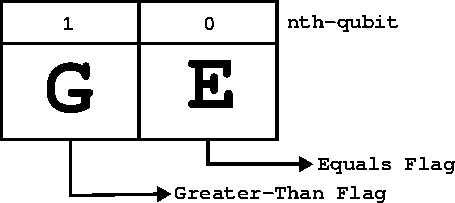
\includegraphics[scale=0.8]{images/6_Complete_System/status_reg_diagram.pdf}
    \caption{The diagram of the Status Quantum registers}
\end{figure}

\begin{listing}[!ht]
    \centering
    \begin{minted}{python3}
        from qiskit import QuantumCircuit, QuantumRegister

        op = QuantumRegister(2, name="Opcode")
        a = QuantumRegister(2, name="A")
        b = QuantumRegister(2, name="B")
        out = QuantumRegister(8, name="Out")
        stat = QuantumRegister(2, name="Status")

        qalu = QuantumCircuit(op, a, b, out, stat)
    \end{minted}
    \caption{The initialization Python code for the Quantum circuit of the Quantum ALU}
\end{listing}

After the initialization of the circuit we have to append each of the Quantum circuits that implement each of the operations
as custom Quantum gates.

To control when each of the operation will be selected accordingly to the opcode bitstring we are going to use the member
method \verb|control()| of the \verb|Gate| class. This function takes numerous parameters but we are going to use only
two of those: the \verb|num_control_qubits| and the \verb|ctrl_state| parameters. The \verb|num_control_qubits| stores
how many qubits will be used control qubits to signal the activation of the gate and the \verb|ctrl_state| parameter
annotates what is the control state of each of the control qubits. For instance, the bitstring \verb|"101"| annotates
that the least-significant and most-significant qubits will be true when in the $\ket{1}$ state and the qubit in position
1 is going to be true in the $\ket{0}$ state (inverse logic).

Using this method it is very easy to map each gate/operation to the appropriate opcode bitstring: \\\verb|ctrl_state="10"| for
the multiplication gate and \verb|ctrl_state="11"| for the comparison gate. We just have to supply the opcode register
when appending.

The addition and subtraction operations where left last because they are not that straig!ht-forward to append. These operations are
implemented by one gate that can change its mode by a control signal as an independent input. The other two operations needed
to set the \verb|num_ctrl_qubits=2| because they did not use a control signal as an input. This means that we can use one qubit
of the opcode register as an input for the Quantum Adder-Subtractor and thus we have to set \verb|num_ctrl_qubits=2| and
\verb|ctrl_state="0"| because according to the opcode table the most-significant qubit of the those operations is always in the
$\ket{0}$ state.

\begin{listing}[!ht]
    \begin{minted}{python3}
        qalu.append(addsub.control(1, ctrl_state="0"),\
            ([op[1]] + [op[0]] + a[:] + b[:] + out[:n+1]))
        qalu.append(mul.control(2, ctrl_state="10"),\
            (op[:] + a[:] + b[:] + out[:]))
        qalu.append(cmp.control(2, ctrl_state="11"),\
            (op[:] + a[:] + b[:] + out[:n+1] + stat[:]))
    \end{minted}
    \caption{Appending the custom Quantum gates of the operations to the Quantum ALU}
\end{listing}

\begin{figure}[!ht]
    \centering
    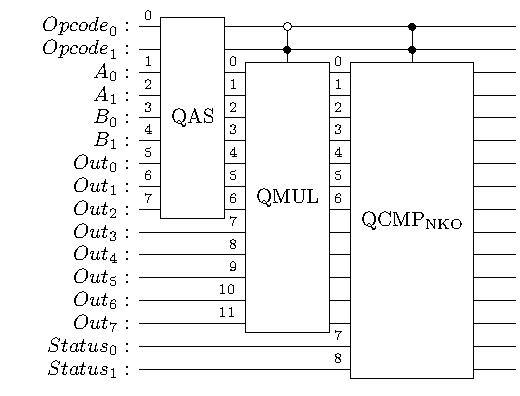
\includegraphics{images/6_Complete_System/qalu_complete.pdf}
    \caption{The Quantum circuit diagram of the Quantum ALU}
\end{figure}
\newpage
\section{Experimental Results on Simulators and Quantum Computers}
\subsection{Testing the Addition and Subtraction operations on the Aer Simulator and on a real Quantum Computer}

We will now demonstrate all of the operations of the Quantum ALU starting with addition and subtraction. Before executing any arithmetic and logic 
operation we have to initialize the Opcode register with the appropriate opcode (see Table 6.1).

Therefore, to perform an addition, the Opcode register must be initialized with the $\ket{00}$ state. For this demonstration
registers A and B are initialized with the states $\ket{11}=\ket{3}$ and $\ket{10}=\ket{2}$ respectively Listing (28):

\begin{listing}[!ht]
        \begin{minted}{python3}
            qalu.x(a[0])
            qalu.x(a[1]) # a = 11
            qalu.x(b[1]) # b = 10
        \end{minted}
        \caption{Initializing the Quantum registers A and B with the appropriate values}
        \label{ls:6_init_add}
\end{listing}

Executing the Quantum ALU circuit on an Aer simulator, the Output register arrives at the state $\ket{00000101}=\ket{5}$ which is the expected value.
In Figure (6.3) we can see this even more clearly (we omitted the five leading zeros for a clearer picture of the result):

\begin{figure}[!ht]
        \centering
        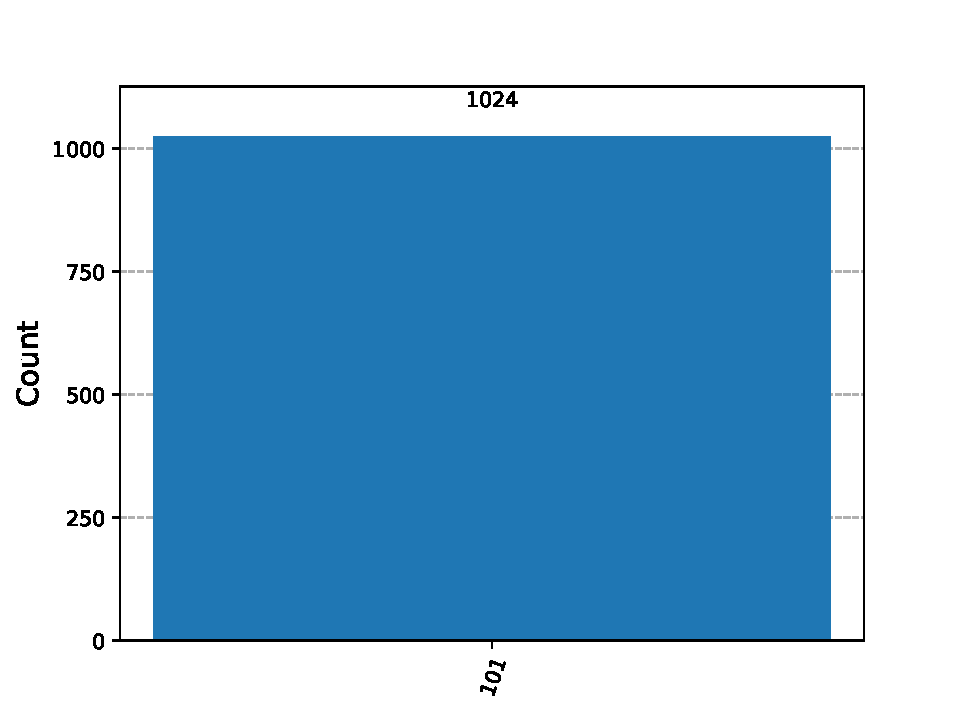
\includegraphics[scale=0.7]{images/6_Complete_System/adder_subtractor_aer_result.pdf}
        \caption{The histogram of the possible values of the Output register when the Quantum ALU performed an addition with A=3 (11) and B=2 (10) on the Aer Simulator}
\end{figure}

We shall now execute a subtraction operation with the same initial values for the A and B registers and submit a job to an IBM Quantum Computer
so that the circuit can be executed. We want to note that the expected output is $101_2$ which can be interpreted in many ways but because
the Adder-Subtractor implements a design where it performs signed and unsigned-mangitude addition and subtraction and because $A \geq B$ the
third qubit of the output register can be omitted thus the result becomes $01_2$ or just $1$ which is the expected output.

Before showing any experimental results, we would like to note that the Aer simulator and the IBM Quantum Computers execute the quantum circuits
multiple times. The Aer simulator executes them 1024 times while the IBM Quantum Computers execute them four times more, or 4096 times. Thus the
probability of the state of a specific quantum register is either obtained by the following equation:

\begin{equation}
    P(o) = \lceil \frac{c}{n}100 \rceil
\end{equation}
where $o$ is the state of the quantum register, $c$ is the \textit{count}, the number of times the specific state was the actual output, and $n$ is the total number
of executions which can be either 1024 (for the Aer simulations) or 4096 (for any IBM Quantum Computer).

In Figure (6.4) we can see multiple expected output values. Although we did not use any gate that puts any qubit in superposition, Quantum Computers
are vulnerable to noise. Noise, just like in classical computers, can cause problems like flipping a single bit's state from example; a memory cell
of a Random Access Memory module. In the case of the Quantum computer, a qubit can be flipped and give erroneous results.

\begin{figure}[!ht]
        \centering
        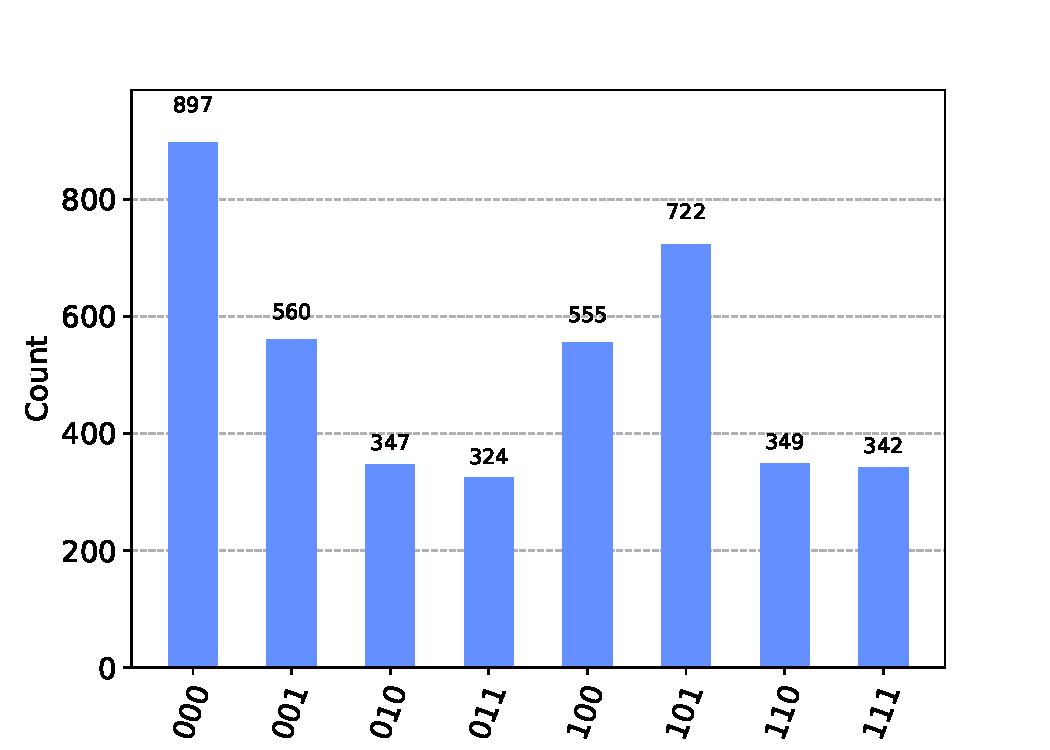
\includegraphics[scale=0.7]{images/6_Complete_System/adder_subtractor_ibmq_result.pdf}
        \caption{The histogram of the possible values of the Output register (with omitted the five leading zero'ed qubits) when the Quantum ALU performed
        an addition with A=3 (11) and B=2 (10) on the IBM Kyoto Quantum Computer}
\end{figure}

We can see that the expected value ($101_2$) has a probability of $17.64\%$ to be output'ed by the circuit.

\newpage
\subsection{Testing the Multiplication operation on the Aer Simulator and on a real Quantum Computer}
We shall demonstrate the multiplication operation with another pair of inputs. This time we shall initialize both A and B with the same value. We
arbitrarily chose $10_2$ or $2_{10}$.

Before anything else, we initialize the Opcode register with the appropriate opcode ($\ket{10}$) and then initialize the A and B registers.

\begin{listing}[!ht]
    \centering
    \begin{minted}{python3}
        qalu.x(op[1]) # op = 10
        qalu.x(a[1])
        qalu.x(b[1])
    \end{minted}
    \caption{The initialization of the Opcode, A and B Quantum registers to perform the multiplication operation}
\end{listing}

The result from the Aer simulator (see Figure (6.5))is what we expected. The result output only shows the qubits 0, 4, 6 and 7.

\begin{figure}[!ht]
    \centering
    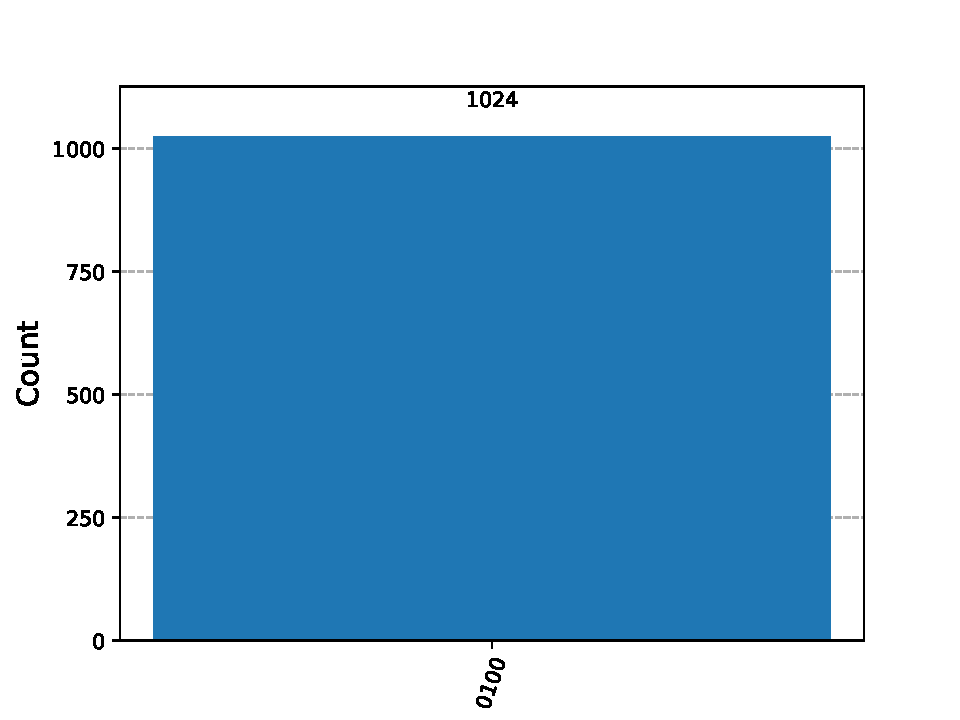
\includegraphics[scale=0.7]{images/6_Complete_System/multiplier_aer_result.pdf}
    \caption{The histogram of the possible values of the Output register when the Quantum ALU performed a multiplication with A=B=2 (10) on the Aer Simulator}
\end{figure}

Executing the same operation on a Quantum computer yields again the same behavior. We get counts of possible outputs instead of a definite answer (see Figure (6.6)).

\begin{figure}[!ht]
        \centering
        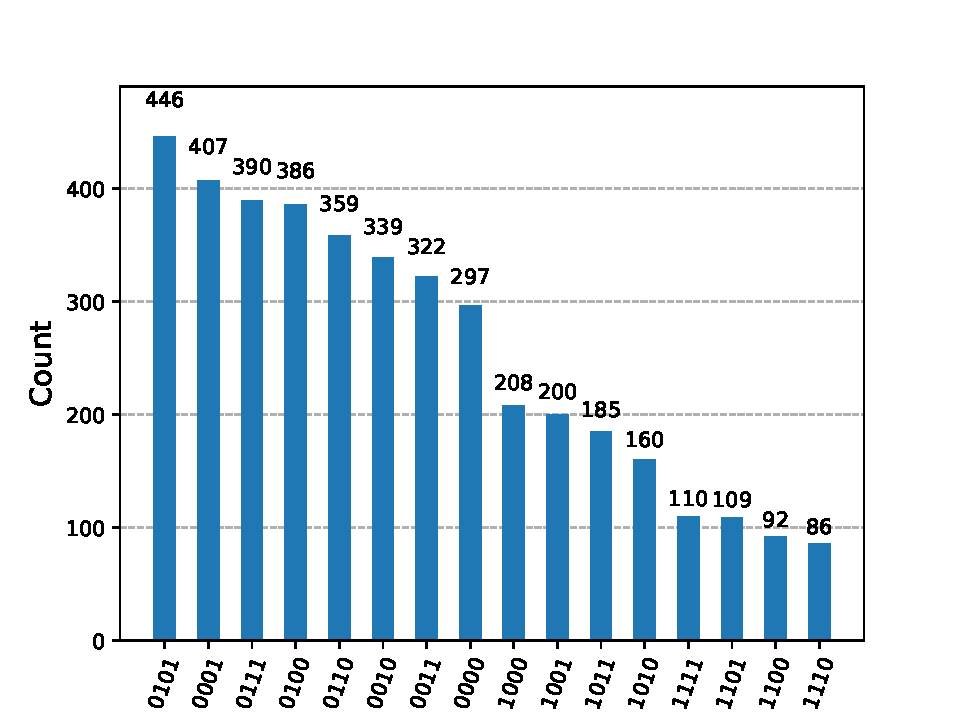
\includegraphics[scale=0.7]{images/6_Complete_System/multiplier_ibmq_result.pdf}
        \caption{The histogram of the possible values of the Output register when the Quantum ALU performed a multiplication with A=B=2 (10) on the IBM Osaka Quantum Computer}
\end{figure}

We note that the expected output ($0100_2=4_{10}$) has a $9.42\%$ probability.

\newpage
\subsection{Testing the Comparison operation on the Aer Simulator and on a real Quantum Computer}
Lastly, we executed the NKO Comparator with the two two-qubit registers inputs A and B to be again $3$ and $2$ respectively and we only measured the two qubits
of the status Quantum register. The execution of the Quantum circuit happened on the IBM Osaka Quantum Computer too. We will again contrast the real-hardware result with the
simulation results.

\begin{figure}[!ht]
    \centering
    \begin{subfigure}{0.5\textwidth}
        \centering
        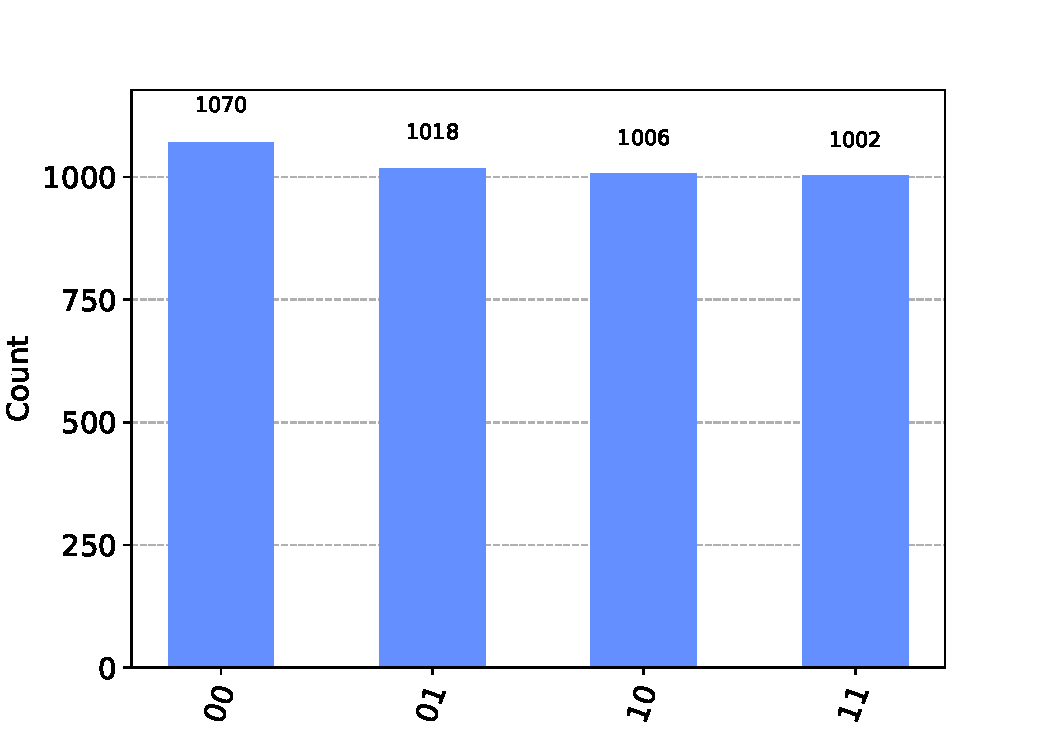
\includegraphics[scale=0.4]{images/6_Complete_System/nko_cmp_ibmq_result.pdf}
        \caption{}    
    \end{subfigure}
    \begin{subfigure}{0.5\textwidth}
        \centering
        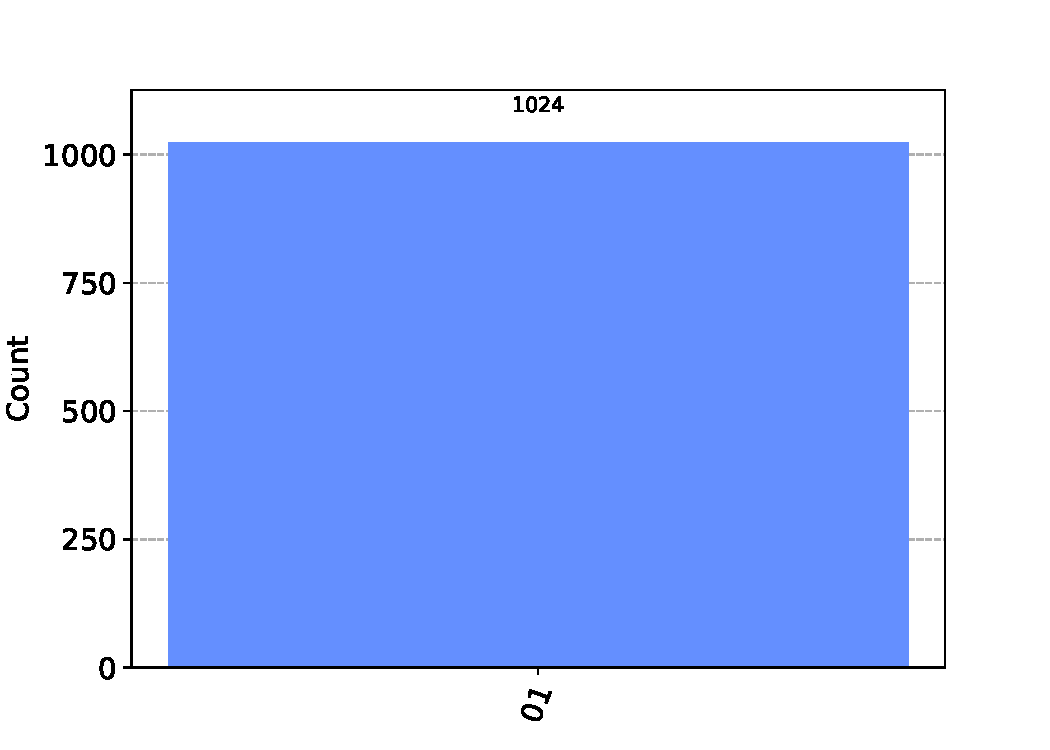
\includegraphics[scale=0.4]{images/6_Complete_System/nko_cmp_aer_result.pdf}
        \caption{}
    \end{subfigure}
    \caption{The results of the comparison operation executed on the IBM Osaka (a) and on the Aer Simulator (b)}
\end{figure}

The same story applies here, where the expected value, output'ed by the Aer Simulator, $10$ which means \say{$A\neq B\text{ and }A \geq B$}, is not the most probable output when executed
4096 times on the Quantum computer. We again compiled a table containing the probability of each output based on how many times the output occured while executing.

\begin{table}[!ht]
    \centering
    \begin{tabular}{c|c|c}
        Output Bit Sequence & Count & Probabilty ($\frac{\text{Count}}{4096}$) \\
        \hline
        $00$ & $1070$ & $26.123\%$ \\
        $01$ & $1018$ & $24.854\%$ \\
        $10$ & $1006$ & $24.561\%$ \\
        $11$ & $1002$ & $24.463\%$ \\
    \end{tabular}
    \caption{The result of probabilities of each output value of the execution of the comparison operation on the IBM Osaka}
\end{table}

We can see that each output has relatively close probability of output meaning that the Quantum computer does not give us a reliable output.
\chapter{The Complete Quantum ALU}

By gathering the previous Quantum circuits we can create the Quantum Arithmetic Logic Unit very easily. Before
we do just that we would like to take a step back and analyse how this Unit may operate.

Just like a classical ALU, the Quantum ALU operates on some general purpose registers and on a register that stores
the status of logic operations. On top of those, the Quantum ALU, may need an \textit{operation code} or \textit{opcode}
to command it to do a specific operation. We shall analyze those opcodes further.

\section{The Quantum ALU's Opcodes}

We had introduced four different Quantum circuits in the previous chapters:
\begin{enumerate}
    \item a Quantum Adder-Subtractor,
    \item a Quantum Multiplier and
    \item a Quantum Comparator
\end{enumerate}
with each Quantum circuit giving us the operations of: addition, subtraction, multiplication and magnitued comparison.
We can encode these four operations using a bitstring of length $n=2$ because $log_24=2$. The mapping of each opcode with
its corresponding operation and Quantum circuit can be seen at the table below.

\begin{table}[!ht]
    \centering
    \begin{tabular}{c|c|c}
        Opcode & Operation & Quantum circuit \\
        \hline
        \verb|00| & Addition & $QAS$ (Addition mode) \\
        \verb|01| & Subtraction & $QAS$ (Subtraction mode) \\
        \verb|10| & Multiplication & $QMUL$ \\
        \verb|11| & Magnitude Comparison & $QCMP_{NKO}$ \\
    \end{tabular}
    \caption{The Opcode table of the Quantum ALU}
\end{table}
\section{The Quantum ALU's circuit}

We will implement the Quantum ALU as any other Quantum circuit we have already presented. This Quantum circuit will have
in total sixteen qubits. The first two-qubit Quantum register is called the \textit{opcode} register and it stores the bitstring
of which operation the Quantum ALU must complete, the two two-qubit general purpose Quantum registers $A$ and $B$ is where
we store the binary encoded numbers we want to be operating, the eig!ht-qubit output Quantum register $Out$ where it is used to
store the output of each operation and lastly, the two-qubit status Quantum register $Status$ where each qubit corresponds to
a logic flag.

\begin{figure}[!ht]
    \centering
    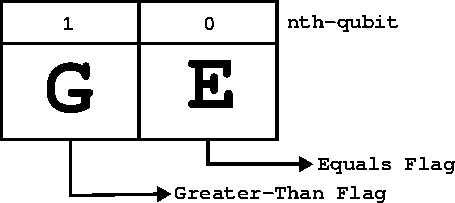
\includegraphics[scale=0.8]{images/6_Complete_System/status_reg_diagram.pdf}
    \caption{The diagram of the Status Quantum registers}
\end{figure}

\begin{listing}[!ht]
    \centering
    \begin{minted}{python3}
        from qiskit import QuantumCircuit, QuantumRegister

        op = QuantumRegister(2, name="Opcode")
        a = QuantumRegister(2, name="A")
        b = QuantumRegister(2, name="B")
        out = QuantumRegister(8, name="Out")
        stat = QuantumRegister(2, name="Status")

        qalu = QuantumCircuit(op, a, b, out, stat)
    \end{minted}
    \caption{The initialization Python code for the Quantum circuit of the Quantum ALU}
\end{listing}

After the initialization of the circuit we have to append each of the Quantum circuits that implement each of the operations
as custom Quantum gates.

To control when each of the operation will be selected accordingly to the opcode bitstring we are going to use the member
method \verb|control()| of the \verb|Gate| class. This function takes numerous parameters but we are going to use only
two of those: the \verb|num_control_qubits| and the \verb|ctrl_state| parameters. The \verb|num_control_qubits| stores
how many qubits will be used control qubits to signal the activation of the gate and the \verb|ctrl_state| parameter
annotates what is the control state of each of the control qubits. For instance, the bitstring \verb|"101"| annotates
that the least-significant and most-significant qubits will be true when in the $\ket{1}$ state and the qubit in position
1 is going to be true in the $\ket{0}$ state (inverse logic).

Using this method it is very easy to map each gate/operation to the appropriate opcode bitstring: \\\verb|ctrl_state="10"| for
the multiplication gate and \verb|ctrl_state="11"| for the comparison gate. We just have to supply the opcode register
when appending.

The addition and subtraction operations where left last because they are not that straig!ht-forward to append. These operations are
implemented by one gate that can change its mode by a control signal as an independent input. The other two operations needed
to set the \verb|num_ctrl_qubits=2| because they did not use a control signal as an input. This means that we can use one qubit
of the opcode register as an input for the Quantum Adder-Subtractor and thus we have to set \verb|num_ctrl_qubits=2| and
\verb|ctrl_state="0"| because according to the opcode table the most-significant qubit of the those operations is always in the
$\ket{0}$ state.

\begin{listing}[!ht]
    \begin{minted}{python3}
        qalu.append(addsub.control(1, ctrl_state="0"),\
            ([op[1]] + [op[0]] + a[:] + b[:] + out[:n+1]))
        qalu.append(mul.control(2, ctrl_state="10"),\
            (op[:] + a[:] + b[:] + out[:]))
        qalu.append(cmp.control(2, ctrl_state="11"),\
            (op[:] + a[:] + b[:] + out[:n+1] + stat[:]))
    \end{minted}
    \caption{Appending the custom Quantum gates of the operations to the Quantum ALU}
\end{listing}

\begin{figure}[!ht]
    \centering
    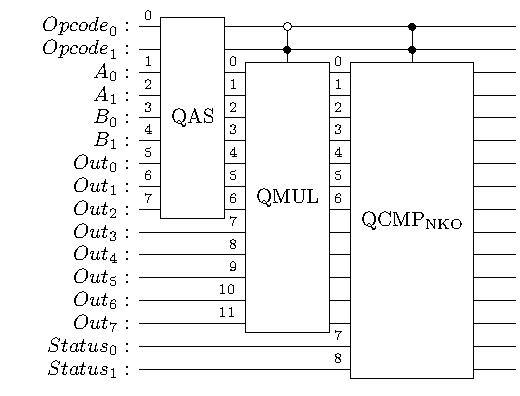
\includegraphics{images/6_Complete_System/qalu_complete.pdf}
    \caption{The Quantum circuit diagram of the Quantum ALU}
\end{figure}
\newpage
\section{Experimental Results on Simulators and Quantum Computers}
\subsection{Testing the Addition and Subtraction operations on the Aer Simulator and on a real Quantum Computer}

We will now demonstrate all of the operations of the Quantum ALU starting with addition and subtraction. Before executing any arithmetic and logic 
operation we have to initialize the Opcode register with the appropriate opcode (see Table 6.1).

Therefore, to perform an addition, the Opcode register must be initialized with the $\ket{00}$ state. For this demonstration
registers A and B are initialized with the states $\ket{11}=\ket{3}$ and $\ket{10}=\ket{2}$ respectively Listing (28):

\begin{listing}[!ht]
        \begin{minted}{python3}
            qalu.x(a[0])
            qalu.x(a[1]) # a = 11
            qalu.x(b[1]) # b = 10
        \end{minted}
        \caption{Initializing the Quantum registers A and B with the appropriate values}
        \label{ls:6_init_add}
\end{listing}

Executing the Quantum ALU circuit on an Aer simulator, the Output register arrives at the state $\ket{00000101}=\ket{5}$ which is the expected value.
In Figure (6.3) we can see this even more clearly (we omitted the five leading zeros for a clearer picture of the result):

\begin{figure}[!ht]
        \centering
        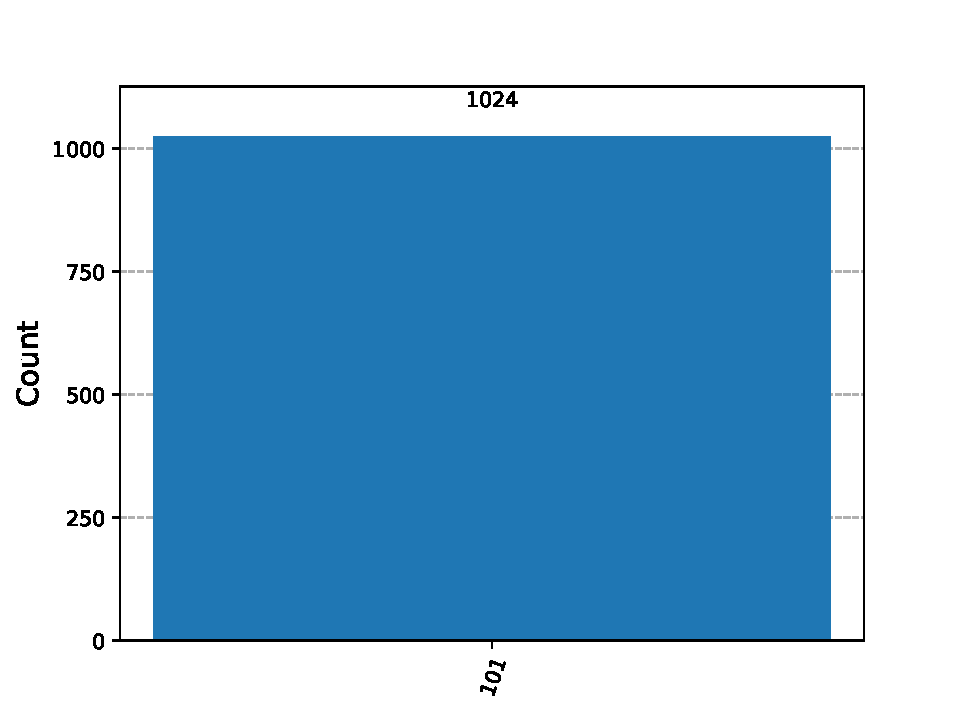
\includegraphics[scale=0.7]{images/6_Complete_System/adder_subtractor_aer_result.pdf}
        \caption{The histogram of the possible values of the Output register when the Quantum ALU performed an addition with A=3 (11) and B=2 (10) on the Aer Simulator}
\end{figure}

We shall now execute a subtraction operation with the same initial values for the A and B registers and submit a job to an IBM Quantum Computer
so that the circuit can be executed. We want to note that the expected output is $101_2$ which can be interpreted in many ways but because
the Adder-Subtractor implements a design where it performs signed and unsigned-mangitude addition and subtraction and because $A \geq B$ the
third qubit of the output register can be omitted thus the result becomes $01_2$ or just $1$ which is the expected output.

Before showing any experimental results, we would like to note that the Aer simulator and the IBM Quantum Computers execute the quantum circuits
multiple times. The Aer simulator executes them 1024 times while the IBM Quantum Computers execute them four times more, or 4096 times. Thus the
probability of the state of a specific quantum register is either obtained by the following equation:

\begin{equation}
    P(o) = \lceil \frac{c}{n}100 \rceil
\end{equation}
where $o$ is the state of the quantum register, $c$ is the \textit{count}, the number of times the specific state was the actual output, and $n$ is the total number
of executions which can be either 1024 (for the Aer simulations) or 4096 (for any IBM Quantum Computer).

In Figure (6.4) we can see multiple expected output values. Although we did not use any gate that puts any qubit in superposition, Quantum Computers
are vulnerable to noise. Noise, just like in classical computers, can cause problems like flipping a single bit's state from example; a memory cell
of a Random Access Memory module. In the case of the Quantum computer, a qubit can be flipped and give erroneous results.

\begin{figure}[!ht]
        \centering
        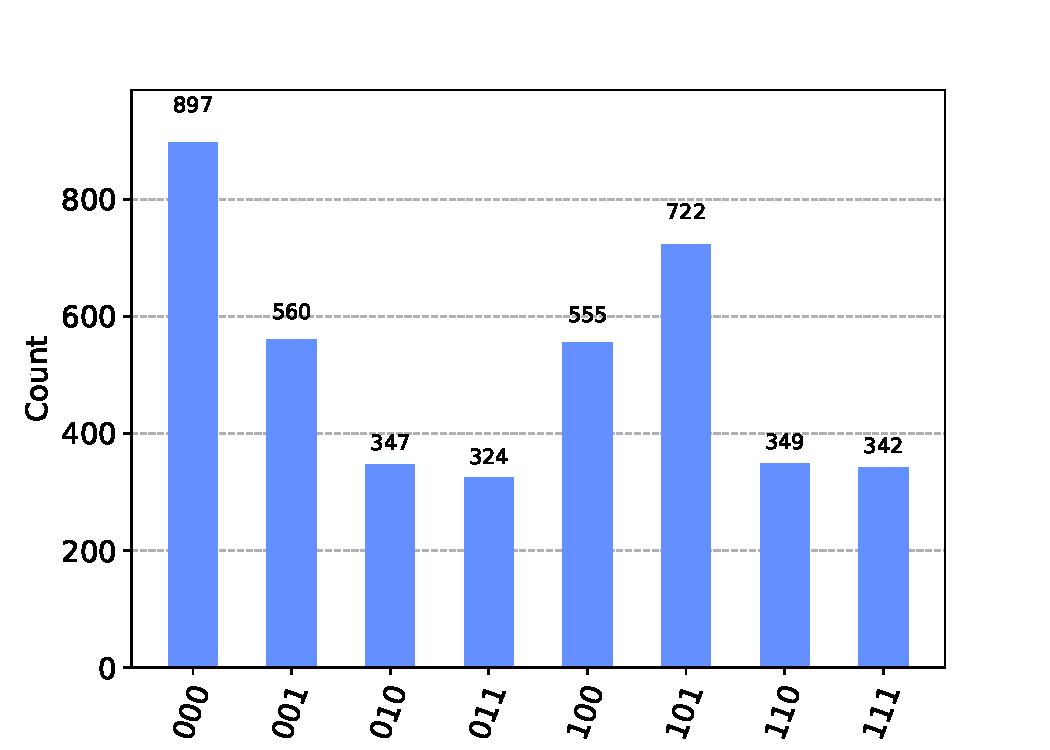
\includegraphics[scale=0.7]{images/6_Complete_System/adder_subtractor_ibmq_result.pdf}
        \caption{The histogram of the possible values of the Output register (with omitted the five leading zero'ed qubits) when the Quantum ALU performed
        an addition with A=3 (11) and B=2 (10) on the IBM Kyoto Quantum Computer}
\end{figure}

We can see that the expected value ($101_2$) has a probability of $17.64\%$ to be output'ed by the circuit.

\newpage
\subsection{Testing the Multiplication operation on the Aer Simulator and on a real Quantum Computer}
We shall demonstrate the multiplication operation with another pair of inputs. This time we shall initialize both A and B with the same value. We
arbitrarily chose $10_2$ or $2_{10}$.

Before anything else, we initialize the Opcode register with the appropriate opcode ($\ket{10}$) and then initialize the A and B registers.

\begin{listing}[!ht]
    \centering
    \begin{minted}{python3}
        qalu.x(op[1]) # op = 10
        qalu.x(a[1])
        qalu.x(b[1])
    \end{minted}
    \caption{The initialization of the Opcode, A and B Quantum registers to perform the multiplication operation}
\end{listing}

The result from the Aer simulator (see Figure (6.5))is what we expected. The result output only shows the qubits 0, 4, 6 and 7.

\begin{figure}[!ht]
    \centering
    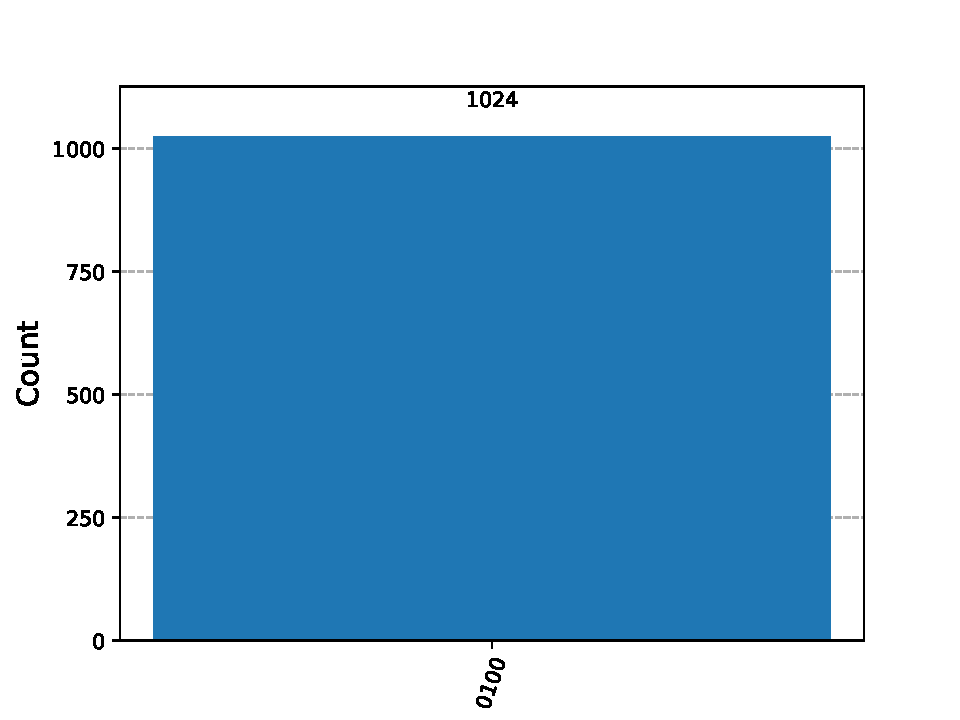
\includegraphics[scale=0.7]{images/6_Complete_System/multiplier_aer_result.pdf}
    \caption{The histogram of the possible values of the Output register when the Quantum ALU performed a multiplication with A=B=2 (10) on the Aer Simulator}
\end{figure}

Executing the same operation on a Quantum computer yields again the same behavior. We get counts of possible outputs instead of a definite answer (see Figure (6.6)).

\begin{figure}[!ht]
        \centering
        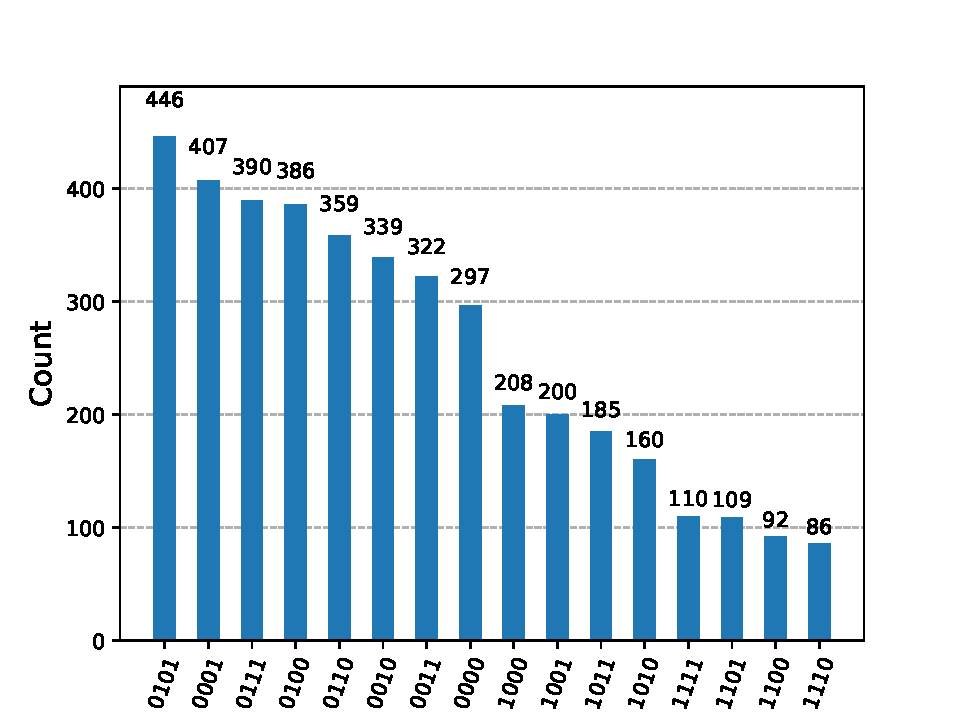
\includegraphics[scale=0.7]{images/6_Complete_System/multiplier_ibmq_result.pdf}
        \caption{The histogram of the possible values of the Output register when the Quantum ALU performed a multiplication with A=B=2 (10) on the IBM Osaka Quantum Computer}
\end{figure}

We note that the expected output ($0100_2=4_{10}$) has a $9.42\%$ probability.

\newpage
\subsection{Testing the Comparison operation on the Aer Simulator and on a real Quantum Computer}
Lastly, we executed the NKO Comparator with the two two-qubit registers inputs A and B to be again $3$ and $2$ respectively and we only measured the two qubits
of the status Quantum register. The execution of the Quantum circuit happened on the IBM Osaka Quantum Computer too. We will again contrast the real-hardware result with the
simulation results.

\begin{figure}[!ht]
    \centering
    \begin{subfigure}{0.5\textwidth}
        \centering
        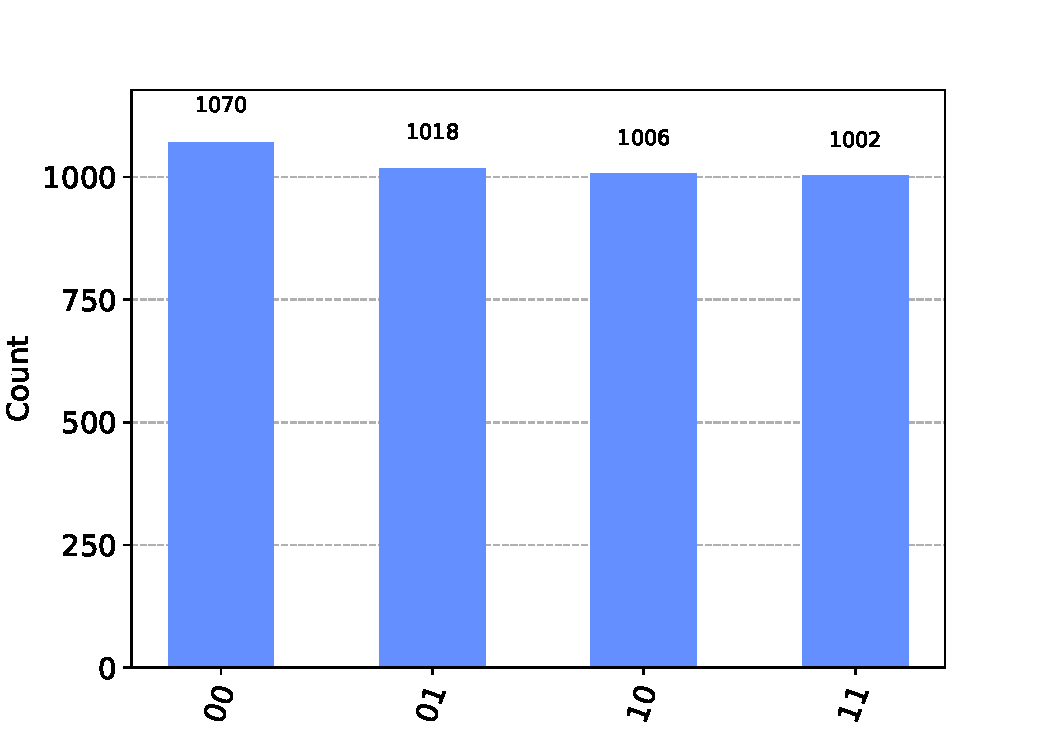
\includegraphics[scale=0.4]{images/6_Complete_System/nko_cmp_ibmq_result.pdf}
        \caption{}    
    \end{subfigure}
    \begin{subfigure}{0.5\textwidth}
        \centering
        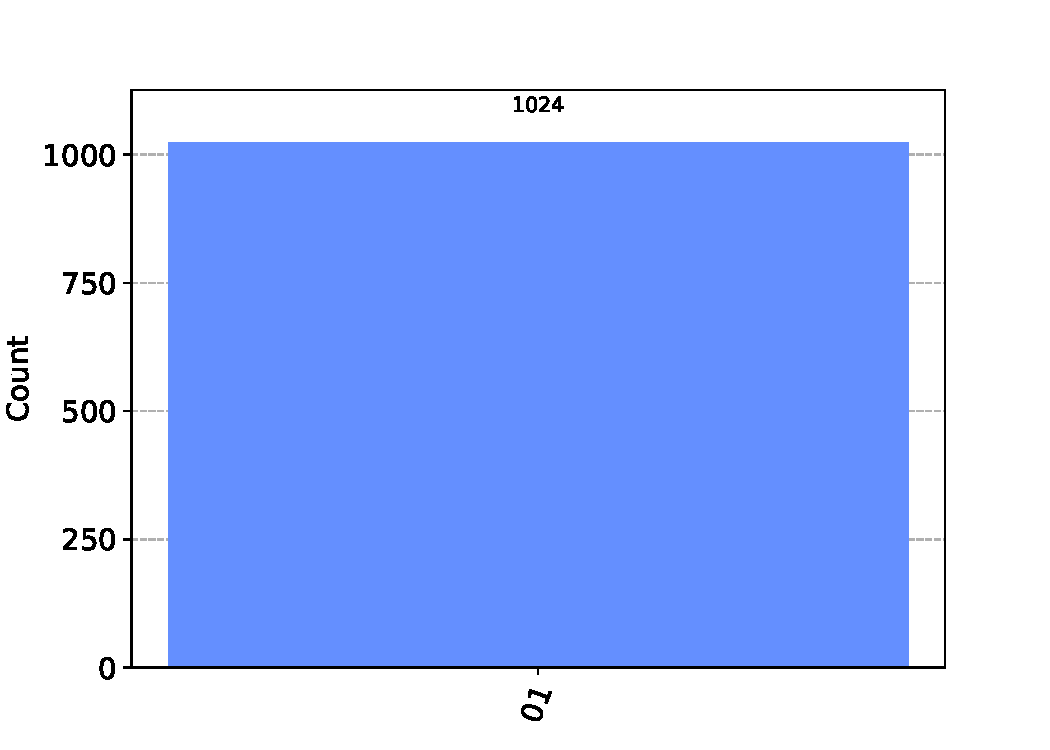
\includegraphics[scale=0.4]{images/6_Complete_System/nko_cmp_aer_result.pdf}
        \caption{}
    \end{subfigure}
    \caption{The results of the comparison operation executed on the IBM Osaka (a) and on the Aer Simulator (b)}
\end{figure}

The same story applies here, where the expected value, output'ed by the Aer Simulator, $10$ which means \say{$A\neq B\text{ and }A \geq B$}, is not the most probable output when executed
4096 times on the Quantum computer. We again compiled a table containing the probability of each output based on how many times the output occured while executing.

\begin{table}[!ht]
    \centering
    \begin{tabular}{c|c|c}
        Output Bit Sequence & Count & Probabilty ($\frac{\text{Count}}{4096}$) \\
        \hline
        $00$ & $1070$ & $26.123\%$ \\
        $01$ & $1018$ & $24.854\%$ \\
        $10$ & $1006$ & $24.561\%$ \\
        $11$ & $1002$ & $24.463\%$ \\
    \end{tabular}
    \caption{The result of probabilities of each output value of the execution of the comparison operation on the IBM Osaka}
\end{table}

We can see that each output has relatively close probability of output meaning that the Quantum computer does not give us a reliable output.
\chapter{The Complete Quantum ALU}

By gathering the previous Quantum circuits we can create the Quantum Arithmetic Logic Unit very easily. Before
we do just that we would like to take a step back and analyse how this Unit may operate.

Just like a classical ALU, the Quantum ALU operates on some general purpose registers and on a register that stores
the status of logic operations. On top of those, the Quantum ALU, may need an \textit{operation code} or \textit{opcode}
to command it to do a specific operation. We shall analyze those opcodes further.

\section{The Quantum ALU's Opcodes}

We had introduced four different Quantum circuits in the previous chapters:
\begin{enumerate}
    \item a Quantum Adder-Subtractor,
    \item a Quantum Multiplier and
    \item a Quantum Comparator
\end{enumerate}
with each Quantum circuit giving us the operations of: addition, subtraction, multiplication and magnitued comparison.
We can encode these four operations using a bitstring of length $n=2$ because $log_24=2$. The mapping of each opcode with
its corresponding operation and Quantum circuit can be seen at the table below.

\begin{table}[!ht]
    \centering
    \begin{tabular}{c|c|c}
        Opcode & Operation & Quantum circuit \\
        \hline
        \verb|00| & Addition & $QAS$ (Addition mode) \\
        \verb|01| & Subtraction & $QAS$ (Subtraction mode) \\
        \verb|10| & Multiplication & $QMUL$ \\
        \verb|11| & Magnitude Comparison & $QCMP_{NKO}$ \\
    \end{tabular}
    \caption{The Opcode table of the Quantum ALU}
\end{table}
\section{The Quantum ALU's circuit}

We will implement the Quantum ALU as any other Quantum circuit we have already presented. This Quantum circuit will have
in total sixteen qubits. The first two-qubit Quantum register is called the \textit{opcode} register and it stores the bitstring
of which operation the Quantum ALU must complete, the two two-qubit general purpose Quantum registers $A$ and $B$ is where
we store the binary encoded numbers we want to be operating, the eig!ht-qubit output Quantum register $Out$ where it is used to
store the output of each operation and lastly, the two-qubit status Quantum register $Status$ where each qubit corresponds to
a logic flag.

\begin{figure}[!ht]
    \centering
    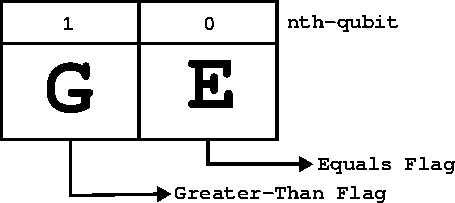
\includegraphics[scale=0.8]{images/6_Complete_System/status_reg_diagram.pdf}
    \caption{The diagram of the Status Quantum registers}
\end{figure}

\begin{listing}[!ht]
    \centering
    \begin{minted}{python3}
        from qiskit import QuantumCircuit, QuantumRegister

        op = QuantumRegister(2, name="Opcode")
        a = QuantumRegister(2, name="A")
        b = QuantumRegister(2, name="B")
        out = QuantumRegister(8, name="Out")
        stat = QuantumRegister(2, name="Status")

        qalu = QuantumCircuit(op, a, b, out, stat)
    \end{minted}
    \caption{The initialization Python code for the Quantum circuit of the Quantum ALU}
\end{listing}

After the initialization of the circuit we have to append each of the Quantum circuits that implement each of the operations
as custom Quantum gates.

To control when each of the operation will be selected accordingly to the opcode bitstring we are going to use the member
method \verb|control()| of the \verb|Gate| class. This function takes numerous parameters but we are going to use only
two of those: the \verb|num_control_qubits| and the \verb|ctrl_state| parameters. The \verb|num_control_qubits| stores
how many qubits will be used control qubits to signal the activation of the gate and the \verb|ctrl_state| parameter
annotates what is the control state of each of the control qubits. For instance, the bitstring \verb|"101"| annotates
that the least-significant and most-significant qubits will be true when in the $\ket{1}$ state and the qubit in position
1 is going to be true in the $\ket{0}$ state (inverse logic).

Using this method it is very easy to map each gate/operation to the appropriate opcode bitstring: \\\verb|ctrl_state="10"| for
the multiplication gate and \verb|ctrl_state="11"| for the comparison gate. We just have to supply the opcode register
when appending.

The addition and subtraction operations where left last because they are not that straig!ht-forward to append. These operations are
implemented by one gate that can change its mode by a control signal as an independent input. The other two operations needed
to set the \verb|num_ctrl_qubits=2| because they did not use a control signal as an input. This means that we can use one qubit
of the opcode register as an input for the Quantum Adder-Subtractor and thus we have to set \verb|num_ctrl_qubits=2| and
\verb|ctrl_state="0"| because according to the opcode table the most-significant qubit of the those operations is always in the
$\ket{0}$ state.

\begin{listing}[!ht]
    \begin{minted}{python3}
        qalu.append(addsub.control(1, ctrl_state="0"),\
            ([op[1]] + [op[0]] + a[:] + b[:] + out[:n+1]))
        qalu.append(mul.control(2, ctrl_state="10"),\
            (op[:] + a[:] + b[:] + out[:]))
        qalu.append(cmp.control(2, ctrl_state="11"),\
            (op[:] + a[:] + b[:] + out[:n+1] + stat[:]))
    \end{minted}
    \caption{Appending the custom Quantum gates of the operations to the Quantum ALU}
\end{listing}

\begin{figure}[!ht]
    \centering
    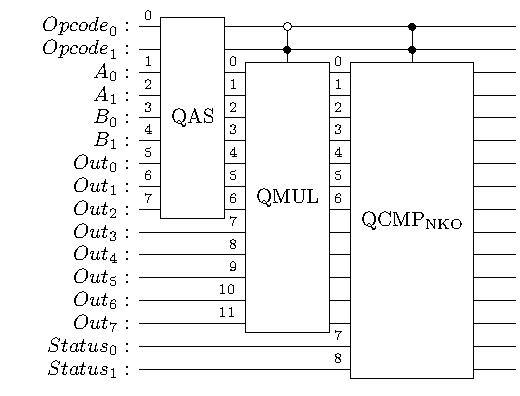
\includegraphics{images/6_Complete_System/qalu_complete.pdf}
    \caption{The Quantum circuit diagram of the Quantum ALU}
\end{figure}
\newpage
\section{Experimental Results on Simulators and Quantum Computers}
\subsection{Testing the Addition and Subtraction operations on the Aer Simulator and on a real Quantum Computer}

We will now demonstrate all of the operations of the Quantum ALU starting with addition and subtraction. Before executing any arithmetic and logic 
operation we have to initialize the Opcode register with the appropriate opcode (see Table 6.1).

Therefore, to perform an addition, the Opcode register must be initialized with the $\ket{00}$ state. For this demonstration
registers A and B are initialized with the states $\ket{11}=\ket{3}$ and $\ket{10}=\ket{2}$ respectively Listing (28):

\begin{listing}[!ht]
        \begin{minted}{python3}
            qalu.x(a[0])
            qalu.x(a[1]) # a = 11
            qalu.x(b[1]) # b = 10
        \end{minted}
        \caption{Initializing the Quantum registers A and B with the appropriate values}
        \label{ls:6_init_add}
\end{listing}

Executing the Quantum ALU circuit on an Aer simulator, the Output register arrives at the state $\ket{00000101}=\ket{5}$ which is the expected value.
In Figure (6.3) we can see this even more clearly (we omitted the five leading zeros for a clearer picture of the result):

\begin{figure}[!ht]
        \centering
        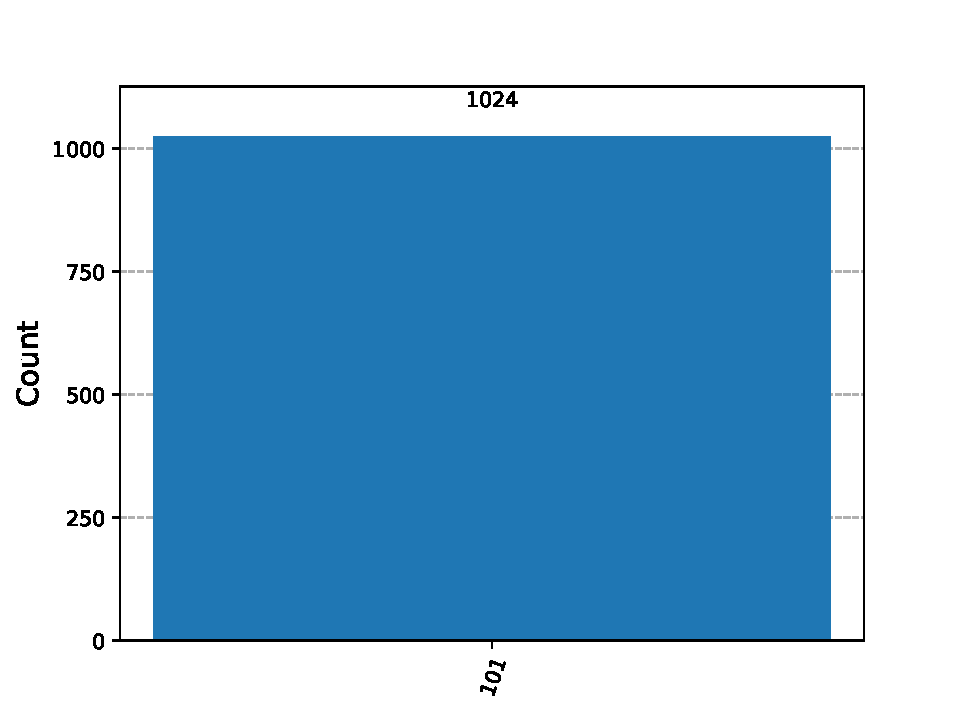
\includegraphics[scale=0.7]{images/6_Complete_System/adder_subtractor_aer_result.pdf}
        \caption{The histogram of the possible values of the Output register when the Quantum ALU performed an addition with A=3 (11) and B=2 (10) on the Aer Simulator}
\end{figure}

We shall now execute a subtraction operation with the same initial values for the A and B registers and submit a job to an IBM Quantum Computer
so that the circuit can be executed. We want to note that the expected output is $101_2$ which can be interpreted in many ways but because
the Adder-Subtractor implements a design where it performs signed and unsigned-mangitude addition and subtraction and because $A \geq B$ the
third qubit of the output register can be omitted thus the result becomes $01_2$ or just $1$ which is the expected output.

Before showing any experimental results, we would like to note that the Aer simulator and the IBM Quantum Computers execute the quantum circuits
multiple times. The Aer simulator executes them 1024 times while the IBM Quantum Computers execute them four times more, or 4096 times. Thus the
probability of the state of a specific quantum register is either obtained by the following equation:

\begin{equation}
    P(o) = \lceil \frac{c}{n}100 \rceil
\end{equation}
where $o$ is the state of the quantum register, $c$ is the \textit{count}, the number of times the specific state was the actual output, and $n$ is the total number
of executions which can be either 1024 (for the Aer simulations) or 4096 (for any IBM Quantum Computer).

In Figure (6.4) we can see multiple expected output values. Although we did not use any gate that puts any qubit in superposition, Quantum Computers
are vulnerable to noise. Noise, just like in classical computers, can cause problems like flipping a single bit's state from example; a memory cell
of a Random Access Memory module. In the case of the Quantum computer, a qubit can be flipped and give erroneous results.

\begin{figure}[!ht]
        \centering
        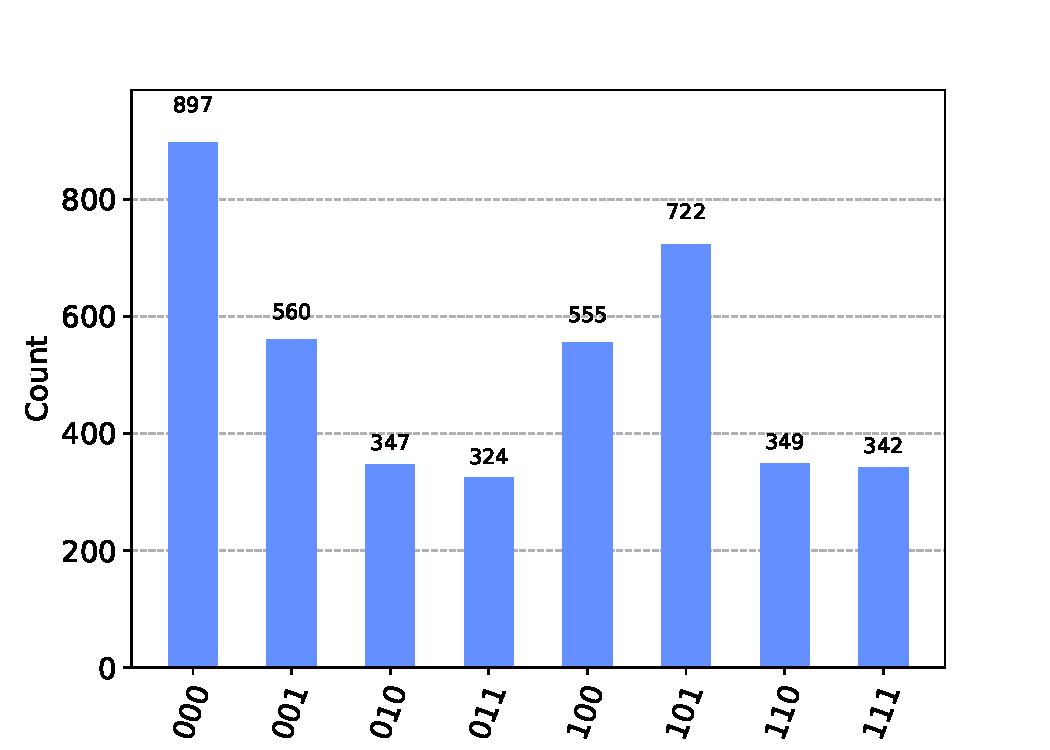
\includegraphics[scale=0.7]{images/6_Complete_System/adder_subtractor_ibmq_result.pdf}
        \caption{The histogram of the possible values of the Output register (with omitted the five leading zero'ed qubits) when the Quantum ALU performed
        an addition with A=3 (11) and B=2 (10) on the IBM Kyoto Quantum Computer}
\end{figure}

We can see that the expected value ($101_2$) has a probability of $17.64\%$ to be output'ed by the circuit.

\newpage
\subsection{Testing the Multiplication operation on the Aer Simulator and on a real Quantum Computer}
We shall demonstrate the multiplication operation with another pair of inputs. This time we shall initialize both A and B with the same value. We
arbitrarily chose $10_2$ or $2_{10}$.

Before anything else, we initialize the Opcode register with the appropriate opcode ($\ket{10}$) and then initialize the A and B registers.

\begin{listing}[!ht]
    \centering
    \begin{minted}{python3}
        qalu.x(op[1]) # op = 10
        qalu.x(a[1])
        qalu.x(b[1])
    \end{minted}
    \caption{The initialization of the Opcode, A and B Quantum registers to perform the multiplication operation}
\end{listing}

The result from the Aer simulator (see Figure (6.5))is what we expected. The result output only shows the qubits 0, 4, 6 and 7.

\begin{figure}[!ht]
    \centering
    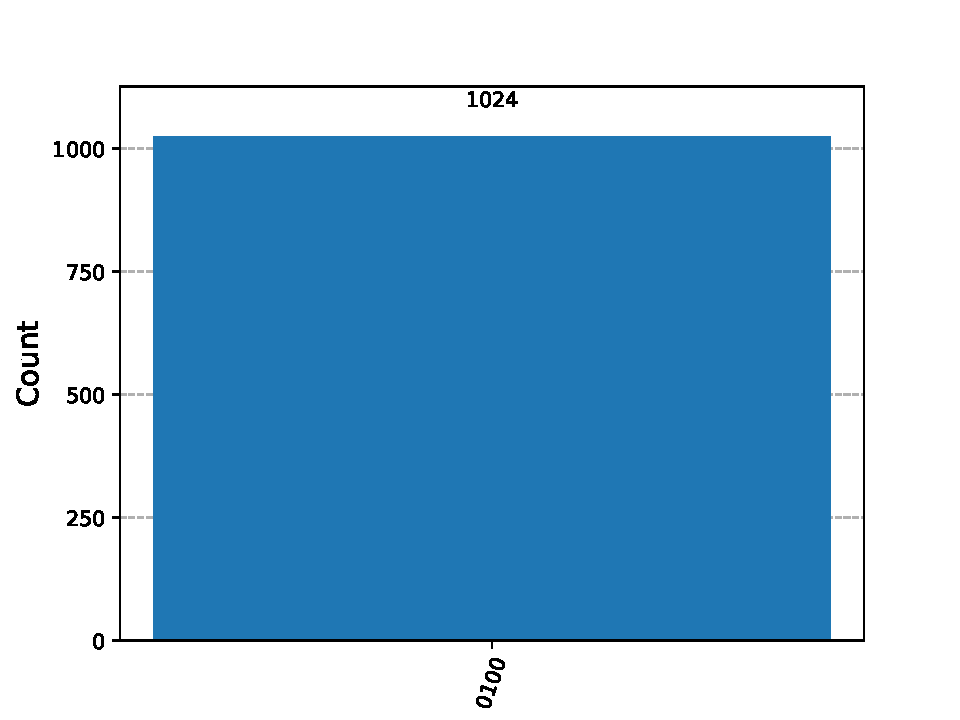
\includegraphics[scale=0.7]{images/6_Complete_System/multiplier_aer_result.pdf}
    \caption{The histogram of the possible values of the Output register when the Quantum ALU performed a multiplication with A=B=2 (10) on the Aer Simulator}
\end{figure}

Executing the same operation on a Quantum computer yields again the same behavior. We get counts of possible outputs instead of a definite answer (see Figure (6.6)).

\begin{figure}[!ht]
        \centering
        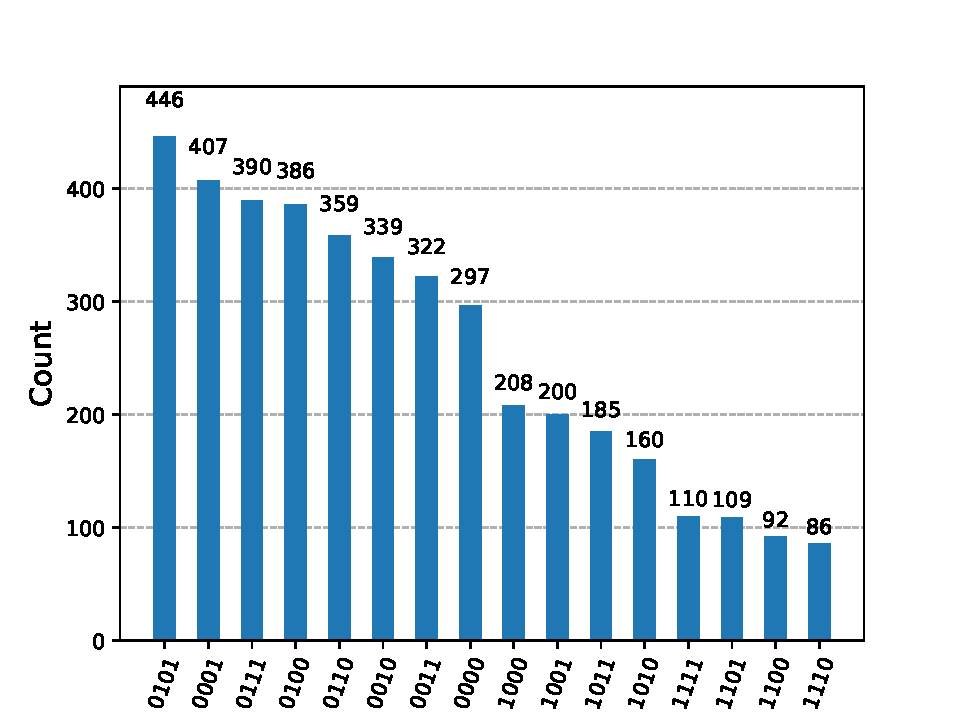
\includegraphics[scale=0.7]{images/6_Complete_System/multiplier_ibmq_result.pdf}
        \caption{The histogram of the possible values of the Output register when the Quantum ALU performed a multiplication with A=B=2 (10) on the IBM Osaka Quantum Computer}
\end{figure}

We note that the expected output ($0100_2=4_{10}$) has a $9.42\%$ probability.

\newpage
\subsection{Testing the Comparison operation on the Aer Simulator and on a real Quantum Computer}
Lastly, we executed the NKO Comparator with the two two-qubit registers inputs A and B to be again $3$ and $2$ respectively and we only measured the two qubits
of the status Quantum register. The execution of the Quantum circuit happened on the IBM Osaka Quantum Computer too. We will again contrast the real-hardware result with the
simulation results.

\begin{figure}[!ht]
    \centering
    \begin{subfigure}{0.5\textwidth}
        \centering
        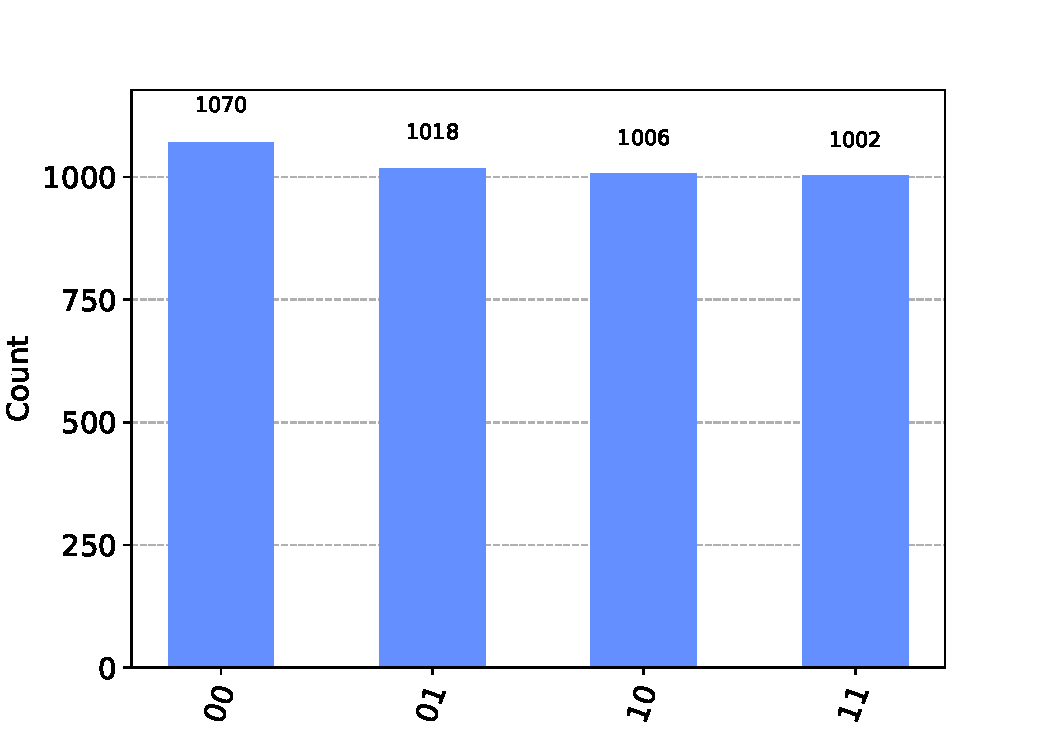
\includegraphics[scale=0.4]{images/6_Complete_System/nko_cmp_ibmq_result.pdf}
        \caption{}    
    \end{subfigure}
    \begin{subfigure}{0.5\textwidth}
        \centering
        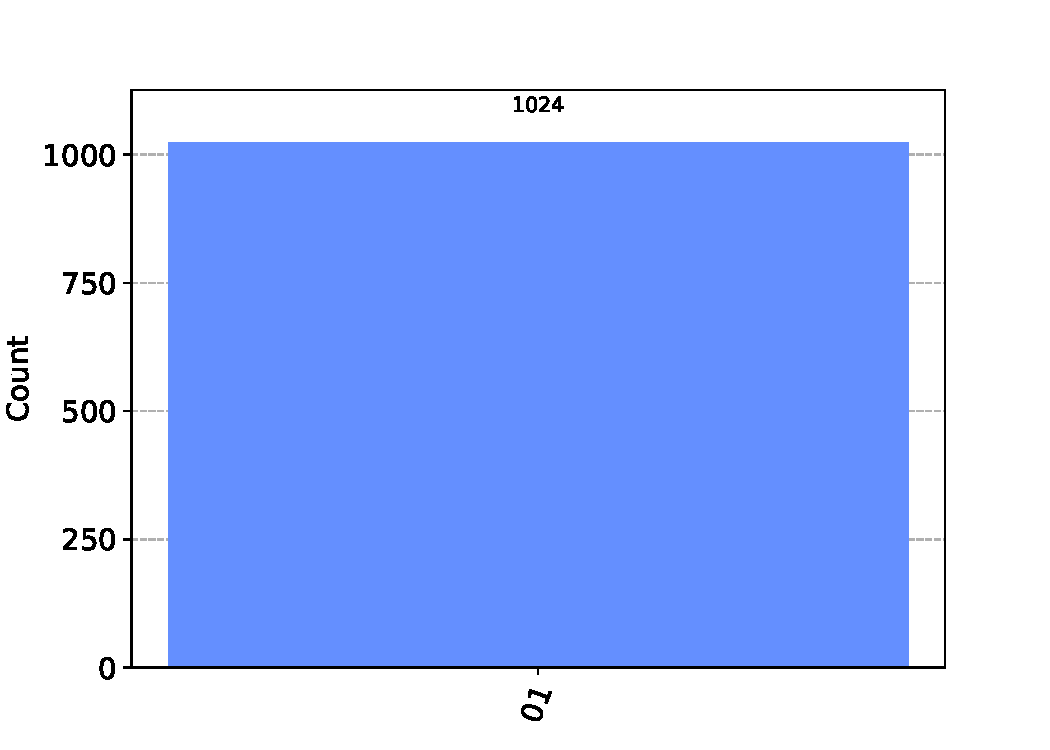
\includegraphics[scale=0.4]{images/6_Complete_System/nko_cmp_aer_result.pdf}
        \caption{}
    \end{subfigure}
    \caption{The results of the comparison operation executed on the IBM Osaka (a) and on the Aer Simulator (b)}
\end{figure}

The same story applies here, where the expected value, output'ed by the Aer Simulator, $10$ which means \say{$A\neq B\text{ and }A \geq B$}, is not the most probable output when executed
4096 times on the Quantum computer. We again compiled a table containing the probability of each output based on how many times the output occured while executing.

\begin{table}[!ht]
    \centering
    \begin{tabular}{c|c|c}
        Output Bit Sequence & Count & Probabilty ($\frac{\text{Count}}{4096}$) \\
        \hline
        $00$ & $1070$ & $26.123\%$ \\
        $01$ & $1018$ & $24.854\%$ \\
        $10$ & $1006$ & $24.561\%$ \\
        $11$ & $1002$ & $24.463\%$ \\
    \end{tabular}
    \caption{The result of probabilities of each output value of the execution of the comparison operation on the IBM Osaka}
\end{table}

We can see that each output has relatively close probability of output meaning that the Quantum computer does not give us a reliable output.
\chapter{The Complete Quantum ALU}

By gathering the previous Quantum circuits we can create the Quantum Arithmetic Logic Unit very easily. Before
we do just that we would like to take a step back and analyse how this Unit may operate.

Just like a classical ALU, the Quantum ALU operates on some general purpose registers and on a register that stores
the status of logic operations. On top of those, the Quantum ALU, may need an \textit{operation code} or \textit{opcode}
to command it to do a specific operation. We shall analyze those opcodes further.

\section{The Quantum ALU's Opcodes}

We had introduced four different Quantum circuits in the previous chapters:
\begin{enumerate}
    \item a Quantum Adder-Subtractor,
    \item a Quantum Multiplier and
    \item a Quantum Comparator
\end{enumerate}
with each Quantum circuit giving us the operations of: addition, subtraction, multiplication and magnitued comparison.
We can encode these four operations using a bitstring of length $n=2$ because $log_24=2$. The mapping of each opcode with
its corresponding operation and Quantum circuit can be seen at the table below.

\begin{table}[!ht]
    \centering
    \begin{tabular}{c|c|c}
        Opcode & Operation & Quantum circuit \\
        \hline
        \verb|00| & Addition & $QAS$ (Addition mode) \\
        \verb|01| & Subtraction & $QAS$ (Subtraction mode) \\
        \verb|10| & Multiplication & $QMUL$ \\
        \verb|11| & Magnitude Comparison & $QCMP_{NKO}$ \\
    \end{tabular}
    \caption{The Opcode table of the Quantum ALU}
\end{table}
\section{The Quantum ALU's circuit}

We will implement the Quantum ALU as any other Quantum circuit we have already presented. This Quantum circuit will have
in total sixteen qubits. The first two-qubit Quantum register is called the \textit{opcode} register and it stores the bitstring
of which operation the Quantum ALU must complete, the two two-qubit general purpose Quantum registers $A$ and $B$ is where
we store the binary encoded numbers we want to be operating, the eig!ht-qubit output Quantum register $Out$ where it is used to
store the output of each operation and lastly, the two-qubit status Quantum register $Status$ where each qubit corresponds to
a logic flag.

\begin{figure}[!ht]
    \centering
    \includegraphics[scale=0.8]{images/6_Complete_System/status_reg_diagram.pdf}
    \caption{The diagram of the Status Quantum registers}
\end{figure}

\begin{listing}[!ht]
    \centering
    \begin{minted}{python3}
        from qiskit import QuantumCircuit, QuantumRegister

        op = QuantumRegister(2, name="Opcode")
        a = QuantumRegister(2, name="A")
        b = QuantumRegister(2, name="B")
        out = QuantumRegister(8, name="Out")
        stat = QuantumRegister(2, name="Status")

        qalu = QuantumCircuit(op, a, b, out, stat)
    \end{minted}
    \caption{The initialization Python code for the Quantum circuit of the Quantum ALU}
\end{listing}

After the initialization of the circuit we have to append each of the Quantum circuits that implement each of the operations
as custom Quantum gates.

To control when each of the operation will be selected accordingly to the opcode bitstring we are going to use the member
method \verb|control()| of the \verb|Gate| class. This function takes numerous parameters but we are going to use only
two of those: the \verb|num_control_qubits| and the \verb|ctrl_state| parameters. The \verb|num_control_qubits| stores
how many qubits will be used control qubits to signal the activation of the gate and the \verb|ctrl_state| parameter
annotates what is the control state of each of the control qubits. For instance, the bitstring \verb|"101"| annotates
that the least-significant and most-significant qubits will be true when in the $\ket{1}$ state and the qubit in position
1 is going to be true in the $\ket{0}$ state (inverse logic).

Using this method it is very easy to map each gate/operation to the appropriate opcode bitstring: \\\verb|ctrl_state="10"| for
the multiplication gate and \verb|ctrl_state="11"| for the comparison gate. We just have to supply the opcode register
when appending.

The addition and subtraction operations where left last because they are not that straig!ht-forward to append. These operations are
implemented by one gate that can change its mode by a control signal as an independent input. The other two operations needed
to set the \verb|num_ctrl_qubits=2| because they did not use a control signal as an input. This means that we can use one qubit
of the opcode register as an input for the Quantum Adder-Subtractor and thus we have to set \verb|num_ctrl_qubits=2| and
\verb|ctrl_state="0"| because according to the opcode table the most-significant qubit of the those operations is always in the
$\ket{0}$ state.

\begin{listing}[!ht]
    \begin{minted}{python3}
        qalu.append(addsub.control(1, ctrl_state="0"),\
            ([op[1]] + [op[0]] + a[:] + b[:] + out[:n+1]))
        qalu.append(mul.control(2, ctrl_state="10"),\
            (op[:] + a[:] + b[:] + out[:]))
        qalu.append(cmp.control(2, ctrl_state="11"),\
            (op[:] + a[:] + b[:] + out[:n+1] + stat[:]))
    \end{minted}
    \caption{Appending the custom Quantum gates of the operations to the Quantum ALU}
\end{listing}

\begin{figure}[!ht]
    \centering
    \includegraphics{images/6_Complete_System/qalu_complete.pdf}
    \caption{The Quantum circuit diagram of the Quantum ALU}
\end{figure}
\newpage
\section{Experimental Results on Simulators and Quantum Computers}
\subsection{Testing the Addition and Subtraction operations on the Aer Simulator and on a real Quantum Computer}

We will now demonstrate all of the operations of the Quantum ALU starting with addition and subtraction. Before executing any arithmetic and logic 
operation we have to initialize the Opcode register with the appropriate opcode (see Table 6.1).

Therefore, to perform an addition, the Opcode register must be initialized with the $\ket{00}$ state. For this demonstration
registers A and B are initialized with the states $\ket{11}=\ket{3}$ and $\ket{10}=\ket{2}$ respectively Listing (28):

\begin{listing}[!ht]
        \begin{minted}{python3}
            qalu.x(a[0])
            qalu.x(a[1]) # a = 11
            qalu.x(b[1]) # b = 10
        \end{minted}
        \caption{Initializing the Quantum registers A and B with the appropriate values}
        \label{ls:6_init_add}
\end{listing}

Executing the Quantum ALU circuit on an Aer simulator, the Output register arrives at the state $\ket{00000101}=\ket{5}$ which is the expected value.
In Figure (6.3) we can see this even more clearly (we omitted the five leading zeros for a clearer picture of the result):

\begin{figure}[!ht]
        \centering
        \includegraphics[scale=0.7]{images/6_Complete_System/adder_subtractor_aer_result.pdf}
        \caption{The histogram of the possible values of the Output register when the Quantum ALU performed an addition with A=3 (11) and B=2 (10) on the Aer Simulator}
\end{figure}

We shall now execute a subtraction operation with the same initial values for the A and B registers and submit a job to an IBM Quantum Computer
so that the circuit can be executed. We want to note that the expected output is $101_2$ which can be interpreted in many ways but because
the Adder-Subtractor implements a design where it performs signed and unsigned-mangitude addition and subtraction and because $A \geq B$ the
third qubit of the output register can be omitted thus the result becomes $01_2$ or just $1$ which is the expected output.

Before showing any experimental results, we would like to note that the Aer simulator and the IBM Quantum Computers execute the quantum circuits
multiple times. The Aer simulator executes them 1024 times while the IBM Quantum Computers execute them four times more, or 4096 times. Thus the
probability of the state of a specific quantum register is either obtained by the following equation:

\begin{equation}
    P(o) = \lceil \frac{c}{n}100 \rceil
\end{equation}
where $o$ is the state of the quantum register, $c$ is the \textit{count}, the number of times the specific state was the actual output, and $n$ is the total number
of executions which can be either 1024 (for the Aer simulations) or 4096 (for any IBM Quantum Computer).

In Figure (6.4) we can see multiple expected output values. Although we did not use any gate that puts any qubit in superposition, Quantum Computers
are vulnerable to noise. Noise, just like in classical computers, can cause problems like flipping a single bit's state from example; a memory cell
of a Random Access Memory module. In the case of the Quantum computer, a qubit can be flipped and give erroneous results.

\begin{figure}[!ht]
        \centering
        \includegraphics[scale=0.7]{images/6_Complete_System/adder_subtractor_ibmq_result.pdf}
        \caption{The histogram of the possible values of the Output register (with omitted the five leading zero'ed qubits) when the Quantum ALU performed
        an addition with A=3 (11) and B=2 (10) on the IBM Kyoto Quantum Computer}
\end{figure}

We can see that the expected value ($101_2$) has a probability of $17.64\%$ to be output'ed by the circuit.

\newpage
\subsection{Testing the Multiplication operation on the Aer Simulator and on a real Quantum Computer}
We shall demonstrate the multiplication operation with another pair of inputs. This time we shall initialize both A and B with the same value. We
arbitrarily chose $10_2$ or $2_{10}$.

Before anything else, we initialize the Opcode register with the appropriate opcode ($\ket{10}$) and then initialize the A and B registers.

\begin{listing}[!ht]
    \centering
    \begin{minted}{python3}
        qalu.x(op[1]) # op = 10
        qalu.x(a[1])
        qalu.x(b[1])
    \end{minted}
    \caption{The initialization of the Opcode, A and B Quantum registers to perform the multiplication operation}
\end{listing}

The result from the Aer simulator (see Figure (6.5))is what we expected. The result output only shows the qubits 0, 4, 6 and 7.

\begin{figure}[!ht]
    \centering
    \includegraphics[scale=0.7]{images/6_Complete_System/multiplier_aer_result.pdf}
    \caption{The histogram of the possible values of the Output register when the Quantum ALU performed a multiplication with A=B=2 (10) on the Aer Simulator}
\end{figure}

Executing the same operation on a Quantum computer yields again the same behavior. We get counts of possible outputs instead of a definite answer (see Figure (6.6)).

\begin{figure}[!ht]
        \centering
        \includegraphics[scale=0.7]{images/6_Complete_System/multiplier_ibmq_result.pdf}
        \caption{The histogram of the possible values of the Output register when the Quantum ALU performed a multiplication with A=B=2 (10) on the IBM Osaka Quantum Computer}
\end{figure}

We note that the expected output ($0100_2=4_{10}$) has a $9.42\%$ probability.

\newpage
\subsection{Testing the Comparison operation on the Aer Simulator and on a real Quantum Computer}
Lastly, we executed the NKO Comparator with the two two-qubit registers inputs A and B to be again $3$ and $2$ respectively and we only measured the two qubits
of the status Quantum register. The execution of the Quantum circuit happened on the IBM Osaka Quantum Computer too. We will again contrast the real-hardware result with the
simulation results.

\begin{figure}[!ht]
    \centering
    \begin{subfigure}{0.5\textwidth}
        \centering
        \includegraphics[scale=0.4]{images/6_Complete_System/nko_cmp_ibmq_result.pdf}
        \caption{}    
    \end{subfigure}
    \begin{subfigure}{0.5\textwidth}
        \centering
        \includegraphics[scale=0.4]{images/6_Complete_System/nko_cmp_aer_result.pdf}
        \caption{}
    \end{subfigure}
    \caption{The results of the comparison operation executed on the IBM Osaka (a) and on the Aer Simulator (b)}
\end{figure}

The same story applies here, where the expected value, output'ed by the Aer Simulator, $10$ which means \say{$A\neq B\text{ and }A \geq B$}, is not the most probable output when executed
4096 times on the Quantum computer. We again compiled a table containing the probability of each output based on how many times the output occured while executing.

\begin{table}[!ht]
    \centering
    \begin{tabular}{c|c|c}
        Output Bit Sequence & Count & Probabilty ($\frac{\text{Count}}{4096}$) \\
        \hline
        $00$ & $1070$ & $26.123\%$ \\
        $01$ & $1018$ & $24.854\%$ \\
        $10$ & $1006$ & $24.561\%$ \\
        $11$ & $1002$ & $24.463\%$ \\
    \end{tabular}
    \caption{The result of probabilities of each output value of the execution of the comparison operation on the IBM Osaka}
\end{table}

We can see that each output has relatively close probability of output meaning that the Quantum computer does not give us a reliable output.

% Bibliography
\bibliographystyle{ieeetr} % Use IEEE Transactions bibliography style
\bibliography{includes/references} % Reference list located in 'includes/references.bib'

\end{document}
